%% bm.pdf preamble - material merged from previous preamble and current pandoc preamable output
% NOTE: float placement required changes to the source files referenced by bm.tex
% May 28, 2020
%
% Use lualatex to compile - test with MiKTeX 2.9

% uncomment to list all files in log
%\listfiles

\documentclass[12pt]{report}


\usepackage{fontspec}

%\setmainfont[Scale=MatchLowercase]{Lucida Bright}
%\setmonofont{FreeMono}
%\setmonofont{Source Code Pro}
\setmonofont[Scale=MatchLowercase]{Ubuntu Mono}

% short snippets of asian languages
\newfontfamily\myAsian{Noto Serif TC Medium}

\usepackage[headings]{fullpage}

% national use characters 
%\usepackage{inputenc}

% ams mathematical symbols
\usepackage{amsmath,amssymb}

% added to support pandoc highlighting
\usepackage{microtype}

\usepackage{makeidx}

% add index and bibliographies to table of contents
\usepackage[nottoc]{tocbibind}

% postscript courier and times in place of cm fonts
%\usepackage{courier}
%\usepackage{times}

% extended coloring
\usepackage{color}
\usepackage[table,dvipsnames]{xcolor}
\usepackage{colortbl}

% advanced date formating
\usepackage{datetime}

%support pandoc code highlighting
\usepackage{fancyvrb}

% \DefineShortVerb[commandchars=\\\{\}]{\|}
% \DefineVerbatimEnvironment{Highlighting}{Verbatim}{commandchars=\\\{\}}
% % Add ',fontsize=\small' for more characters per line

% tango style colors
% \usepackage{framed}
% \definecolor{shadecolor}{RGB}{255,255,255}
% \newenvironment{Shaded}{\begin{snugshade}}{\end{snugshade}}
% \newcommand{\KeywordTok}[1]{\textcolor[rgb]{0.13,0.29,0.53}{\textbf{{#1}}}}
% \newcommand{\DataTypeTok}[1]{\textcolor[rgb]{0.13,0.29,0.53}{{#1}}}
% \newcommand{\DecValTok}[1]{\textcolor[rgb]{0.00,0.00,0.81}{{#1}}}
% \newcommand{\BaseNTok}[1]{\textcolor[rgb]{0.00,0.00,0.81}{{#1}}}
% \newcommand{\FloatTok}[1]{\textcolor[rgb]{0.00,0.00,0.81}{{#1}}}
% \newcommand{\CharTok}[1]{\textcolor[rgb]{0.31,0.60,0.02}{{#1}}}
% \newcommand{\StringTok}[1]{\textcolor[rgb]{0.31,0.60,0.02}{{#1}}}
% \newcommand{\CommentTok}[1]{\textcolor[rgb]{0.56,0.35,0.01}{\textit{{#1}}}}
% \newcommand{\OtherTok}[1]{\textcolor[rgb]{0.56,0.35,0.01}{{#1}}}
% \newcommand{\AlertTok}[1]{\textcolor[rgb]{0.94,0.16,0.16}{{#1}}}
% \newcommand{\FunctionTok}[1]{\textcolor[rgb]{0.00,0.00,0.00}{{#1}}}
% \newcommand{\RegionMarkerTok}[1]{{#1}}
% \newcommand{\ErrorTok}[1]{\textbf{{#1}}}
% \newcommand{\NormalTok}[1]{{#1}}

% %espresso style colors
% \usepackage{framed}
% \definecolor{shadecolor}{RGB}{42,33,28}
% \newenvironment{Shaded}{\begin{snugshade}}{\end{snugshade}}
% \newcommand{\KeywordTok}[1]{\textcolor[rgb]{0.26,0.66,0.93}{\textbf{{#1}}}}
% \newcommand{\DataTypeTok}[1]{\textcolor[rgb]{0.74,0.68,0.62}{\underline{{#1}}}}
% \newcommand{\DecValTok}[1]{\textcolor[rgb]{0.27,0.67,0.26}{{#1}}}
% \newcommand{\BaseNTok}[1]{\textcolor[rgb]{0.27,0.67,0.26}{{#1}}}
% \newcommand{\FloatTok}[1]{\textcolor[rgb]{0.27,0.67,0.26}{{#1}}}
% \newcommand{\CharTok}[1]{\textcolor[rgb]{0.02,0.61,0.04}{{#1}}}
% \newcommand{\StringTok}[1]{\textcolor[rgb]{0.02,0.61,0.04}{{#1}}}
% \newcommand{\CommentTok}[1]{\textcolor[rgb]{0.00,0.40,1.00}{\textit{{#1}}}}
% \newcommand{\OtherTok}[1]{\textcolor[rgb]{0.74,0.68,0.62}{{#1}}}
% \newcommand{\AlertTok}[1]{\textcolor[rgb]{1.00,1.00,0.00}{{#1}}}
% \newcommand{\FunctionTok}[1]{\textcolor[rgb]{1.00,0.58,0.35}{\textbf{{#1}}}}
% \newcommand{\RegionMarkerTok}[1]{\textcolor[rgb]{0.74,0.68,0.62}{{#1}}}
% \newcommand{\ErrorTok}[1]{\textcolor[rgb]{0.74,0.68,0.62}{\textbf{{#1}}}}
% \newcommand{\NormalTok}[1]{\textcolor[rgb]{0.74,0.68,0.62}{{#1}}}

% %kete style colors
% \newenvironment{Shaded}{}{}
% \newcommand{\KeywordTok}[1]{\textbf{{#1}}}
% \newcommand{\DataTypeTok}[1]{\textcolor[rgb]{0.50,0.00,0.00}{{#1}}}
% \newcommand{\DecValTok}[1]{\textcolor[rgb]{0.00,0.00,1.00}{{#1}}}
% \newcommand{\BaseNTok}[1]{\textcolor[rgb]{0.00,0.00,1.00}{{#1}}}
% \newcommand{\FloatTok}[1]{\textcolor[rgb]{0.50,0.00,0.50}{{#1}}}
% \newcommand{\CharTok}[1]{\textcolor[rgb]{1.00,0.00,1.00}{{#1}}}
% \newcommand{\StringTok}[1]{\textcolor[rgb]{0.87,0.00,0.00}{{#1}}}
% \newcommand{\CommentTok}[1]{\textcolor[rgb]{0.50,0.50,0.50}{\textit{{#1}}}}
% \newcommand{\OtherTok}[1]{{#1}}
% \newcommand{\AlertTok}[1]{\textcolor[rgb]{0.00,1.00,0.00}{\textbf{{#1}}}}
% \newcommand{\FunctionTok}[1]{\textcolor[rgb]{0.00,0.00,0.50}{{#1}}}
% \newcommand{\RegionMarkerTok}[1]{{#1}}
% \newcommand{\ErrorTok}[1]{\textcolor[rgb]{1.00,0.00,0.00}{\textbf{{#1}}}}
% \newcommand{\NormalTok}[1]{{#1}}
% %end pandoc code hacks

% jodliterate colors
\usepackage{color}
\definecolor{shadecolor}{RGB}{248,248,248}
% j control structures 
\definecolor{keywcolor}{rgb}{0.13,0.29,0.53}
% j explicit arguments x y m n u v
\definecolor{datacolor}{rgb}{0.13,0.29,0.53}
% j numbers - all types see j.xml
\definecolor{decvcolor}{rgb}{0.00,0.00,0.81}
\definecolor{basencolor}{rgb}{0.00,0.00,0.81}
\definecolor{floatcolor}{rgb}{0.00,0.00,0.81}
% j local assignments
\definecolor{charcolor}{rgb}{0.31,0.60,0.02}
\definecolor{stringcolor}{rgb}{0.31,0.60,0.02}
\definecolor{commentcolor}{rgb}{0.56,0.35,0.01}
% primitive adverbs and conjunctions
%\definecolor{othercolor}{rgb}{0.56,0.35,0.01}   
\definecolor{othercolor}{RGB}{0,0,255}
% global assignments
\definecolor{alertcolor}{rgb}{0.94,0.16,0.16}
% primitive J verbs and noun names
\definecolor{funccolor}{rgb}{0.00,0.00,0.00}

% custom colors
\definecolor{CodeBackGround}{cmyk}{0.0,0.0,0,0.05}    % light gray
\definecolor{CodeComment}{rgb}{0,0.50,0.00}           % dark green {0,0.45,0.08}
\definecolor{TableStripes}{gray}{0.9}                 % odd/even background in tables

% Colors for the hyperref package
\definecolor{urlcolor}{rgb}{0,.145,.698}
\definecolor{linkcolor}{rgb}{.71,0.21,0.01}
\definecolor{citecolor}{rgb}{.12,.54,.11}

% % Exact colors from NB
\definecolor{incolor}{HTML}{303F9F}
\definecolor{outcolor}{HTML}{D84315}
\definecolor{cellborder}{HTML}{CFCFCF}
\definecolor{cellbackground}{HTML}{F7F7F7}

% % ANSI colors
\definecolor{ansi-black}{HTML}{3E424D}
\definecolor{ansi-black-intense}{HTML}{282C36}
\definecolor{ansi-red}{HTML}{E75C58}
\definecolor{ansi-red-intense}{HTML}{B22B31}
\definecolor{ansi-green}{HTML}{00A250}
\definecolor{ansi-green-intense}{HTML}{007427}
\definecolor{ansi-yellow}{HTML}{DDB62B}
\definecolor{ansi-yellow-intense}{HTML}{B27D12}
\definecolor{ansi-blue}{HTML}{208FFB}
\definecolor{ansi-blue-intense}{HTML}{0065CA}
\definecolor{ansi-magenta}{HTML}{D160C4}
\definecolor{ansi-magenta-intense}{HTML}{A03196}
\definecolor{ansi-cyan}{HTML}{60C6C8}
\definecolor{ansi-cyan-intense}{HTML}{258F8F}
\definecolor{ansi-white}{HTML}{C5C1B4}
\definecolor{ansi-white-intense}{HTML}{A1A6B2}
\definecolor{ansi-default-inverse-fg}{HTML}{FFFFFF}
\definecolor{ansi-default-inverse-bg}{HTML}{000000}
    

% \usepackage{framed}
% \newenvironment{Shaded}{}{}
% \newcommand{\KeywordTok}[1]{\textcolor{keywcolor}{\textbf{{#1}}}}
% \newcommand{\DataTypeTok}[1]{\textcolor{datacolor}{{#1}}}
% %\newcommand{\DecValTok}[1]{\textcolor{decvcolor}{{#1}}}
% \newcommand{\DecValTok}[1]{{#1}} 
% \newcommand{\BaseNTok}[1]{\textcolor{basencolor}{{#1}}}
% \newcommand{\FloatTok}[1]{\textcolor{floatcolor}{{#1}}}
% \newcommand{\CharTok}[1]{\textcolor{charcolor}{\textbf{{#1}}}}
% \newcommand{\StringTok}[1]{\textcolor{stringcolor}{{#1}}}
% \newcommand{\CommentTok}[1]{\textcolor{commentcolor}{\textit{{#1}}}}
% \newcommand{\OtherTok}[1]{\textcolor{othercolor}{{#1}}} 
% \newcommand{\AlertTok}[1]{\textcolor{alertcolor}{\textbf{{#1}}}}
% %\newcommand{\FunctionTok}[1]{\textcolor{funccolor}{{#1}}}
% \newcommand{\FunctionTok}[1]{{#1}}
% \newcommand{\RegionMarkerTok}[1]{{#1}}
% \newcommand{\ErrorTok}[1]{\textbf{{#1}}}
% \newcommand{\NormalTok}[1]{{#1}}

% The default LaTeX title has an obnoxious amount of whitespace. By default,
% titling removes some of it. It also provides customization options.
\usepackage{titling}

% headers and footers
\usepackage{fancyhdr}
%\pagestyle{fancy}
\pagestyle{plain}

\fancyhead{}
\fancyfoot{}

%\fancyhead[LE,RO]{\slshape \rightmark}
%\fancyhead[LO,RE]{\slshape \leftmark}
\fancyfoot[C]{\thepage}
%\headrulewidth 0.4pt
%\footrulewidth 0 pt

%\addtolength{\headheight}{\baselineskip}

%\lfoot{\emph{Analyze the Data not the Drivel}}
%\rfoot{\emph{\today}}

% subfigure handles figures that contain subfigures
%\usepackage{color,graphicx,subfigure,sidecap}
\usepackage{graphicx,sidecap}
\usepackage{subfigure}
\graphicspath{{./inclusions/}}

% floatflt provides for text wrapping around small figures and tables
\usepackage{floatflt}

% tweak caption formats 
\usepackage{caption} 
\usepackage{sidecap}
%\usepackage{subcaption} % not compatible with subfigure

\usepackage{rotating} % flip tables sideways

% complex footnotes
%\usepackage{bigfoot}

% weird logos \XeLaTeX
\usepackage{metalogo}

\newcommand{\HRule}{\rule{\linewidth}{0.5mm}}

\usepackage[breakable]{tcolorbox}

\usepackage{parskip} % Stop auto-indenting (to mimic markdown behaviour)
    
% Basic figure setup, for now with no caption control since it's done
% automatically by Pandoc (which extracts ![](path) syntax from Markdown).
\usepackage{graphicx}

%\DeclareCaptionFormat{nocaption}{}
%\captionsetup{format=nocaption,aboveskip=0pt,belowskip=0pt}

\usepackage[Export]{adjustbox} % Used to constrain images to a maximum size
\adjustboxset{max size={0.9\linewidth}{0.9\paperheight}}
\usepackage{float}

%\floatplacement{figure}{H} % forces figures to be placed at the correct location

\usepackage{xcolor} % Allow colors to be defined
\usepackage{enumerate} % Needed for markdown enumerations to work
\usepackage{geometry} % Used to adjust the document margins

%\usepackage{amsmath} % Equations
%\usepackage{amssymb} % Equations

\usepackage{textcomp} % defines textquotesingle

% Hack from http://tex.stackexchange.com/a/47451/13684:
\AtBeginDocument{%
	\def\PYZsq{\textquotesingle}% Upright quotes in Pygmentized code
}

\usepackage{upquote} % Upright quotes for verbatim code
\usepackage{eurosym} % defines \euro
\usepackage[mathletters]{ucs} % Extended unicode (utf-8) support

%\usepackage{fancyvrb} % verbatim replacement that allows latex

\usepackage{grffile} % extends the file name processing of package graphics 
					 % to support a larger range
					 
\makeatletter % fix for grffile with XeLaTeX
\def\Gread@@xetex#1{%
  \IfFileExists{"\Gin@base".bb}%
  {\Gread@eps{\Gin@base.bb}}%
  {\Gread@@xetex@aux#1}%
}
\makeatother

% The hyperref package gives us a pdf with properly built
% internal navigation ('pdf bookmarks' for the table of contents,
% internal cross-reference links, web links for URLs, etc.)
\usepackage{hyperref}
% The default LaTeX title has an obnoxious amount of whitespace. By default,
% titling removes some of it. It also provides customization options.
\usepackage{titling}
\usepackage{longtable} % longtable support required by pandoc >1.10
\usepackage{booktabs}  % table support for pandoc > 1.12.2
\usepackage[inline]{enumitem} % IRkernel/repr support (it uses the enumerate* environment)
\usepackage[normalem]{ulem} % ulem is needed to support strikethroughs (\sout)
							% normalem makes italics be italics, not underlines
\usepackage{mathrsfs}

% commands and environments needed by pandoc snippets
% extracted from the output of `pandoc -s`
\providecommand{\tightlist}{%
  \setlength{\itemsep}{0pt}\setlength{\parskip}{0pt}}
  
\DefineVerbatimEnvironment{Highlighting}{Verbatim}{commandchars=\\\{\}}
% Add ',fontsize=\small' for more characters per line
\newenvironment{Shaded}{}{}
\newcommand{\KeywordTok}[1]{\textcolor[rgb]{0.00,0.44,0.13}{\textbf{{#1}}}}
\newcommand{\DataTypeTok}[1]{\textcolor[rgb]{0.56,0.13,0.00}{{#1}}}
\newcommand{\DecValTok}[1]{\textcolor[rgb]{0.25,0.63,0.44}{{#1}}}
\newcommand{\BaseNTok}[1]{\textcolor[rgb]{0.25,0.63,0.44}{{#1}}}
\newcommand{\FloatTok}[1]{\textcolor[rgb]{0.25,0.63,0.44}{{#1}}}
\newcommand{\CharTok}[1]{\textcolor[rgb]{0.25,0.44,0.63}{{#1}}}
\newcommand{\StringTok}[1]{\textcolor[rgb]{0.25,0.44,0.63}{{#1}}}
\newcommand{\CommentTok}[1]{\textcolor[rgb]{0.38,0.63,0.69}{\textit{{#1}}}}
\newcommand{\OtherTok}[1]{\textcolor[rgb]{0.00,0.44,0.13}{{#1}}}
\newcommand{\AlertTok}[1]{\textcolor[rgb]{1.00,0.00,0.00}{\textbf{{#1}}}}
\newcommand{\FunctionTok}[1]{\textcolor[rgb]{0.02,0.16,0.49}{{#1}}}
\newcommand{\RegionMarkerTok}[1]{{#1}}
\newcommand{\ErrorTok}[1]{\textcolor[rgb]{1.00,0.00,0.00}{\textbf{{#1}}}}
\newcommand{\NormalTok}[1]{{#1}}

% Additional commands for more recent versions of Pandoc
\newcommand{\ConstantTok}[1]{\textcolor[rgb]{0.53,0.00,0.00}{{#1}}}
\newcommand{\SpecialCharTok}[1]{\textcolor[rgb]{0.25,0.44,0.63}{{#1}}}
\newcommand{\VerbatimStringTok}[1]{\textcolor[rgb]{0.25,0.44,0.63}{{#1}}}
\newcommand{\SpecialStringTok}[1]{\textcolor[rgb]{0.73,0.40,0.53}{{#1}}}
\newcommand{\ImportTok}[1]{{#1}}
\newcommand{\DocumentationTok}[1]{\textcolor[rgb]{0.73,0.13,0.13}{\textit{{#1}}}}
\newcommand{\AnnotationTok}[1]{\textcolor[rgb]{0.38,0.63,0.69}{\textbf{\textit{{#1}}}}}
\newcommand{\CommentVarTok}[1]{\textcolor[rgb]{0.38,0.63,0.69}{\textbf{\textit{{#1}}}}}
\newcommand{\VariableTok}[1]{\textcolor[rgb]{0.10,0.09,0.49}{{#1}}}
\newcommand{\ControlFlowTok}[1]{\textcolor[rgb]{0.00,0.44,0.13}{\textbf{{#1}}}}
\newcommand{\OperatorTok}[1]{\textcolor[rgb]{0.40,0.40,0.40}{{#1}}}
\newcommand{\BuiltInTok}[1]{{#1}}
\newcommand{\ExtensionTok}[1]{{#1}}
\newcommand{\PreprocessorTok}[1]{\textcolor[rgb]{0.74,0.48,0.00}{{#1}}}
\newcommand{\AttributeTok}[1]{\textcolor[rgb]{0.49,0.56,0.16}{{#1}}}
\newcommand{\InformationTok}[1]{\textcolor[rgb]{0.38,0.63,0.69}{\textbf{\textit{{#1}}}}}
\newcommand{\WarningTok}[1]{\textcolor[rgb]{0.38,0.63,0.69}{\textbf{\textit{{#1}}}}}

% Define a nice break command that doesn't care if a line doesn't already exist.
\def\br{\hspace*{\fill} \\* }
% Math Jax compatibility definitions
\def\gt{>}
\def\lt{<}
\let\Oldtex\TeX
\let\Oldlatex\LaTeX
\renewcommand{\TeX}{\textrm{\Oldtex}}
\renewcommand{\LaTeX}{\textrm{\Oldlatex}}
 
% Pygments definitions
\makeatletter
\def\PY@reset{\let\PY@it=\relax \let\PY@bf=\relax%
    \let\PY@ul=\relax \let\PY@tc=\relax%
    \let\PY@bc=\relax \let\PY@ff=\relax}
\def\PY@tok#1{\csname PY@tok@#1\endcsname}
\def\PY@toks#1+{\ifx\relax#1\empty\else%
    \PY@tok{#1}\expandafter\PY@toks\fi}
\def\PY@do#1{\PY@bc{\PY@tc{\PY@ul{%
    \PY@it{\PY@bf{\PY@ff{#1}}}}}}}
\def\PY#1#2{\PY@reset\PY@toks#1+\relax+\PY@do{#2}}

\expandafter\def\csname PY@tok@w\endcsname{\def\PY@tc##1{\textcolor[rgb]{0.73,0.73,0.73}{##1}}}
\expandafter\def\csname PY@tok@c\endcsname{\let\PY@it=\textit\def\PY@tc##1{\textcolor[rgb]{0.25,0.50,0.50}{##1}}}
\expandafter\def\csname PY@tok@cp\endcsname{\def\PY@tc##1{\textcolor[rgb]{0.74,0.48,0.00}{##1}}}
\expandafter\def\csname PY@tok@k\endcsname{\let\PY@bf=\textbf\def\PY@tc##1{\textcolor[rgb]{0.00,0.50,0.00}{##1}}}
\expandafter\def\csname PY@tok@kp\endcsname{\def\PY@tc##1{\textcolor[rgb]{0.00,0.50,0.00}{##1}}}
\expandafter\def\csname PY@tok@kt\endcsname{\def\PY@tc##1{\textcolor[rgb]{0.69,0.00,0.25}{##1}}}
\expandafter\def\csname PY@tok@o\endcsname{\def\PY@tc##1{\textcolor[rgb]{0.40,0.40,0.40}{##1}}}
\expandafter\def\csname PY@tok@ow\endcsname{\let\PY@bf=\textbf\def\PY@tc##1{\textcolor[rgb]{0.67,0.13,1.00}{##1}}}
\expandafter\def\csname PY@tok@nb\endcsname{\def\PY@tc##1{\textcolor[rgb]{0.00,0.50,0.00}{##1}}}
\expandafter\def\csname PY@tok@nf\endcsname{\def\PY@tc##1{\textcolor[rgb]{0.00,0.00,1.00}{##1}}}
\expandafter\def\csname PY@tok@nc\endcsname{\let\PY@bf=\textbf\def\PY@tc##1{\textcolor[rgb]{0.00,0.00,1.00}{##1}}}
\expandafter\def\csname PY@tok@nn\endcsname{\let\PY@bf=\textbf\def\PY@tc##1{\textcolor[rgb]{0.00,0.00,1.00}{##1}}}
\expandafter\def\csname PY@tok@ne\endcsname{\let\PY@bf=\textbf\def\PY@tc##1{\textcolor[rgb]{0.82,0.25,0.23}{##1}}}
\expandafter\def\csname PY@tok@nv\endcsname{\def\PY@tc##1{\textcolor[rgb]{0.10,0.09,0.49}{##1}}}
\expandafter\def\csname PY@tok@no\endcsname{\def\PY@tc##1{\textcolor[rgb]{0.53,0.00,0.00}{##1}}}
\expandafter\def\csname PY@tok@nl\endcsname{\def\PY@tc##1{\textcolor[rgb]{0.63,0.63,0.00}{##1}}}
\expandafter\def\csname PY@tok@ni\endcsname{\let\PY@bf=\textbf\def\PY@tc##1{\textcolor[rgb]{0.60,0.60,0.60}{##1}}}
\expandafter\def\csname PY@tok@na\endcsname{\def\PY@tc##1{\textcolor[rgb]{0.49,0.56,0.16}{##1}}}
\expandafter\def\csname PY@tok@nt\endcsname{\let\PY@bf=\textbf\def\PY@tc##1{\textcolor[rgb]{0.00,0.50,0.00}{##1}}}
\expandafter\def\csname PY@tok@nd\endcsname{\def\PY@tc##1{\textcolor[rgb]{0.67,0.13,1.00}{##1}}}
\expandafter\def\csname PY@tok@s\endcsname{\def\PY@tc##1{\textcolor[rgb]{0.73,0.13,0.13}{##1}}}
\expandafter\def\csname PY@tok@sd\endcsname{\let\PY@it=\textit\def\PY@tc##1{\textcolor[rgb]{0.73,0.13,0.13}{##1}}}
\expandafter\def\csname PY@tok@si\endcsname{\let\PY@bf=\textbf\def\PY@tc##1{\textcolor[rgb]{0.73,0.40,0.53}{##1}}}
\expandafter\def\csname PY@tok@se\endcsname{\let\PY@bf=\textbf\def\PY@tc##1{\textcolor[rgb]{0.73,0.40,0.13}{##1}}}
\expandafter\def\csname PY@tok@sr\endcsname{\def\PY@tc##1{\textcolor[rgb]{0.73,0.40,0.53}{##1}}}
\expandafter\def\csname PY@tok@ss\endcsname{\def\PY@tc##1{\textcolor[rgb]{0.10,0.09,0.49}{##1}}}
\expandafter\def\csname PY@tok@sx\endcsname{\def\PY@tc##1{\textcolor[rgb]{0.00,0.50,0.00}{##1}}}
\expandafter\def\csname PY@tok@m\endcsname{\def\PY@tc##1{\textcolor[rgb]{0.40,0.40,0.40}{##1}}}
\expandafter\def\csname PY@tok@gh\endcsname{\let\PY@bf=\textbf\def\PY@tc##1{\textcolor[rgb]{0.00,0.00,0.50}{##1}}}
\expandafter\def\csname PY@tok@gu\endcsname{\let\PY@bf=\textbf\def\PY@tc##1{\textcolor[rgb]{0.50,0.00,0.50}{##1}}}
\expandafter\def\csname PY@tok@gd\endcsname{\def\PY@tc##1{\textcolor[rgb]{0.63,0.00,0.00}{##1}}}
\expandafter\def\csname PY@tok@gi\endcsname{\def\PY@tc##1{\textcolor[rgb]{0.00,0.63,0.00}{##1}}}
\expandafter\def\csname PY@tok@gr\endcsname{\def\PY@tc##1{\textcolor[rgb]{1.00,0.00,0.00}{##1}}}
\expandafter\def\csname PY@tok@ge\endcsname{\let\PY@it=\textit}
\expandafter\def\csname PY@tok@gs\endcsname{\let\PY@bf=\textbf}
\expandafter\def\csname PY@tok@gp\endcsname{\let\PY@bf=\textbf\def\PY@tc##1{\textcolor[rgb]{0.00,0.00,0.50}{##1}}}
\expandafter\def\csname PY@tok@go\endcsname{\def\PY@tc##1{\textcolor[rgb]{0.53,0.53,0.53}{##1}}}
\expandafter\def\csname PY@tok@gt\endcsname{\def\PY@tc##1{\textcolor[rgb]{0.00,0.27,0.87}{##1}}}
\expandafter\def\csname PY@tok@err\endcsname{\def\PY@bc##1{\setlength{\fboxsep}{0pt}\fcolorbox[rgb]{1.00,0.00,0.00}{1,1,1}{\strut ##1}}}
\expandafter\def\csname PY@tok@kc\endcsname{\let\PY@bf=\textbf\def\PY@tc##1{\textcolor[rgb]{0.00,0.50,0.00}{##1}}}
\expandafter\def\csname PY@tok@kd\endcsname{\let\PY@bf=\textbf\def\PY@tc##1{\textcolor[rgb]{0.00,0.50,0.00}{##1}}}
\expandafter\def\csname PY@tok@kn\endcsname{\let\PY@bf=\textbf\def\PY@tc##1{\textcolor[rgb]{0.00,0.50,0.00}{##1}}}
\expandafter\def\csname PY@tok@kr\endcsname{\let\PY@bf=\textbf\def\PY@tc##1{\textcolor[rgb]{0.00,0.50,0.00}{##1}}}
\expandafter\def\csname PY@tok@bp\endcsname{\def\PY@tc##1{\textcolor[rgb]{0.00,0.50,0.00}{##1}}}
\expandafter\def\csname PY@tok@fm\endcsname{\def\PY@tc##1{\textcolor[rgb]{0.00,0.00,1.00}{##1}}}
\expandafter\def\csname PY@tok@vc\endcsname{\def\PY@tc##1{\textcolor[rgb]{0.10,0.09,0.49}{##1}}}
\expandafter\def\csname PY@tok@vg\endcsname{\def\PY@tc##1{\textcolor[rgb]{0.10,0.09,0.49}{##1}}}
\expandafter\def\csname PY@tok@vi\endcsname{\def\PY@tc##1{\textcolor[rgb]{0.10,0.09,0.49}{##1}}}
\expandafter\def\csname PY@tok@vm\endcsname{\def\PY@tc##1{\textcolor[rgb]{0.10,0.09,0.49}{##1}}}
\expandafter\def\csname PY@tok@sa\endcsname{\def\PY@tc##1{\textcolor[rgb]{0.73,0.13,0.13}{##1}}}
\expandafter\def\csname PY@tok@sb\endcsname{\def\PY@tc##1{\textcolor[rgb]{0.73,0.13,0.13}{##1}}}
\expandafter\def\csname PY@tok@sc\endcsname{\def\PY@tc##1{\textcolor[rgb]{0.73,0.13,0.13}{##1}}}
\expandafter\def\csname PY@tok@dl\endcsname{\def\PY@tc##1{\textcolor[rgb]{0.73,0.13,0.13}{##1}}}
\expandafter\def\csname PY@tok@s2\endcsname{\def\PY@tc##1{\textcolor[rgb]{0.73,0.13,0.13}{##1}}}
\expandafter\def\csname PY@tok@sh\endcsname{\def\PY@tc##1{\textcolor[rgb]{0.73,0.13,0.13}{##1}}}
\expandafter\def\csname PY@tok@s1\endcsname{\def\PY@tc##1{\textcolor[rgb]{0.73,0.13,0.13}{##1}}}
\expandafter\def\csname PY@tok@mb\endcsname{\def\PY@tc##1{\textcolor[rgb]{0.40,0.40,0.40}{##1}}}
\expandafter\def\csname PY@tok@mf\endcsname{\def\PY@tc##1{\textcolor[rgb]{0.40,0.40,0.40}{##1}}}
\expandafter\def\csname PY@tok@mh\endcsname{\def\PY@tc##1{\textcolor[rgb]{0.40,0.40,0.40}{##1}}}
\expandafter\def\csname PY@tok@mi\endcsname{\def\PY@tc##1{\textcolor[rgb]{0.40,0.40,0.40}{##1}}}
\expandafter\def\csname PY@tok@il\endcsname{\def\PY@tc##1{\textcolor[rgb]{0.40,0.40,0.40}{##1}}}
\expandafter\def\csname PY@tok@mo\endcsname{\def\PY@tc##1{\textcolor[rgb]{0.40,0.40,0.40}{##1}}}
\expandafter\def\csname PY@tok@ch\endcsname{\let\PY@it=\textit\def\PY@tc##1{\textcolor[rgb]{0.25,0.50,0.50}{##1}}}
\expandafter\def\csname PY@tok@cm\endcsname{\let\PY@it=\textit\def\PY@tc##1{\textcolor[rgb]{0.25,0.50,0.50}{##1}}}
\expandafter\def\csname PY@tok@cpf\endcsname{\let\PY@it=\textit\def\PY@tc##1{\textcolor[rgb]{0.25,0.50,0.50}{##1}}}
\expandafter\def\csname PY@tok@c1\endcsname{\let\PY@it=\textit\def\PY@tc##1{\textcolor[rgb]{0.25,0.50,0.50}{##1}}}
\expandafter\def\csname PY@tok@cs\endcsname{\let\PY@it=\textit\def\PY@tc##1{\textcolor[rgb]{0.25,0.50,0.50}{##1}}}

\def\PYZbs{\char`\\}
\def\PYZus{\char`\_}
\def\PYZob{\char`\{}
\def\PYZcb{\char`\}}
\def\PYZca{\char`\^}
\def\PYZam{\char`\&}
\def\PYZlt{\char`\<}
\def\PYZgt{\char`\>}
\def\PYZsh{\char`\#}
\def\PYZpc{\char`\%}
\def\PYZdl{\char`\$}
\def\PYZhy{\char`\-}
\def\PYZsq{\char`\'}
\def\PYZdq{\char`\"}
\def\PYZti{\char`\~}
% for compatibility with earlier versions
\def\PYZat{@}
\def\PYZlb{[}
\def\PYZrb{]}
\makeatother

% For linebreaks inside Verbatim environment from package fancyvrb. 
\makeatletter
	\newbox\Wrappedcontinuationbox 
	\newbox\Wrappedvisiblespacebox 
	\newcommand*\Wrappedvisiblespace {\textcolor{red}{\textvisiblespace}} 
	\newcommand*\Wrappedcontinuationsymbol {\textcolor{red}{\llap{\tiny$\m@th\hookrightarrow$}}} 
	\newcommand*\Wrappedcontinuationindent {3ex } 
	\newcommand*\Wrappedafterbreak {\kern\Wrappedcontinuationindent\copy\Wrappedcontinuationbox} 
	% Take advantage of the already applied Pygments mark-up to insert 
	% potential linebreaks for TeX processing. 
	%        {, <, #, %, $, ' and ": go to next line. 
	%        _, }, ^, &, >, - and ~: stay at end of broken line. 
	% Use of \textquotesingle for straight quote. 
	\newcommand*\Wrappedbreaksatspecials {% 
		\def\PYGZus{\discretionary{\char`\_}{\Wrappedafterbreak}{\char`\_}}% 
		\def\PYGZob{\discretionary{}{\Wrappedafterbreak\char`\{}{\char`\{}}% 
		\def\PYGZcb{\discretionary{\char`\}}{\Wrappedafterbreak}{\char`\}}}% 
		\def\PYGZca{\discretionary{\char`\^}{\Wrappedafterbreak}{\char`\^}}% 
		\def\PYGZam{\discretionary{\char`\&}{\Wrappedafterbreak}{\char`\&}}% 
		\def\PYGZlt{\discretionary{}{\Wrappedafterbreak\char`\<}{\char`\<}}% 
		\def\PYGZgt{\discretionary{\char`\>}{\Wrappedafterbreak}{\char`\>}}% 
		\def\PYGZsh{\discretionary{}{\Wrappedafterbreak\char`\#}{\char`\#}}% 
		\def\PYGZpc{\discretionary{}{\Wrappedafterbreak\char`\%}{\char`\%}}% 
		\def\PYGZdl{\discretionary{}{\Wrappedafterbreak\char`\$}{\char`\$}}% 
		\def\PYGZhy{\discretionary{\char`\-}{\Wrappedafterbreak}{\char`\-}}% 
		\def\PYGZsq{\discretionary{}{\Wrappedafterbreak\textquotesingle}{\textquotesingle}}% 
		\def\PYGZdq{\discretionary{}{\Wrappedafterbreak\char`\"}{\char`\"}}% 
		\def\PYGZti{\discretionary{\char`\~}{\Wrappedafterbreak}{\char`\~}}% 
	} 
	% Some characters . , ; ? ! / are not pygmentized. 
	% This macro makes them "active" and they will insert potential linebreaks 
	\newcommand*\Wrappedbreaksatpunct {% 
		\lccode`\~`\.\lowercase{\def~}{\discretionary{\hbox{\char`\.}}{\Wrappedafterbreak}{\hbox{\char`\.}}}% 
		\lccode`\~`\,\lowercase{\def~}{\discretionary{\hbox{\char`\,}}{\Wrappedafterbreak}{\hbox{\char`\,}}}% 
		\lccode`\~`\;\lowercase{\def~}{\discretionary{\hbox{\char`\;}}{\Wrappedafterbreak}{\hbox{\char`\;}}}% 
		\lccode`\~`\:\lowercase{\def~}{\discretionary{\hbox{\char`\:}}{\Wrappedafterbreak}{\hbox{\char`\:}}}% 
		\lccode`\~`\?\lowercase{\def~}{\discretionary{\hbox{\char`\?}}{\Wrappedafterbreak}{\hbox{\char`\?}}}% 
		\lccode`\~`\!\lowercase{\def~}{\discretionary{\hbox{\char`\!}}{\Wrappedafterbreak}{\hbox{\char`\!}}}% 
		\lccode`\~`\/\lowercase{\def~}{\discretionary{\hbox{\char`\/}}{\Wrappedafterbreak}{\hbox{\char`\/}}}% 
		\catcode`\.\active
		\catcode`\,\active 
		\catcode`\;\active
		\catcode`\:\active
		\catcode`\?\active
		\catcode`\!\active
		\catcode`\/\active 
		\lccode`\~`\~ 	
	}
\makeatother

\let\OriginalVerbatim=\Verbatim
\makeatletter
\renewcommand{\Verbatim}[1][1]{%
	%\parskip\z@skip
	\sbox\Wrappedcontinuationbox {\Wrappedcontinuationsymbol}%
	\sbox\Wrappedvisiblespacebox {\FV@SetupFont\Wrappedvisiblespace}%
	\def\FancyVerbFormatLine ##1{\hsize\linewidth
		\vtop{\raggedright\hyphenpenalty\z@\exhyphenpenalty\z@
			\doublehyphendemerits\z@\finalhyphendemerits\z@
			\strut ##1\strut}%
	}%
	% If the linebreak is at a space, the latter will be displayed as visible
	% space at end of first line, and a continuation symbol starts next line.
	% Stretch/shrink are however usually zero for typewriter font.
	\def\FV@Space {%
		\nobreak\hskip\z@ plus\fontdimen3\font minus\fontdimen4\font
		\discretionary{\copy\Wrappedvisiblespacebox}{\Wrappedafterbreak}
		{\kern\fontdimen2\font}%
	}%
	
	% Allow breaks at special characters using \PYG... macros.
	\Wrappedbreaksatspecials
	% Breaks at punctuation characters . , ; ? ! and / need catcode=\active 	
	\OriginalVerbatim[#1,codes*=\Wrappedbreaksatpunct]%
}
\makeatother


% prompt
\makeatletter
\newcommand{\boxspacing}{\kern\kvtcb@left@rule\kern\kvtcb@boxsep}
\makeatother
\newcommand{\prompt}[4]{
	\ttfamily\llap{{\color{#2}[#3]:\hspace{3pt}#4}}\vspace{-\baselineskip}
}
    

% Prevent overflowing lines due to hard-to-break entities
\sloppy 

% Setup hyperref package
\hypersetup{
  breaklinks=true,  % so long urls are correctly broken across lines
  colorlinks=true,
  urlcolor=urlcolor,
  linkcolor=linkcolor,
  citecolor=citecolor,
  pdfauthor={John D. Baker},
  pdftitle={Analyze the Data not the Drivel},
  pdfsubject={Blog},
  pdfcreator={MikTeX+LaTeXe},
  pdfkeywords={blog,wordpress},
  }
  
% Slightly bigger margins than the latex defaults
% \geometry{verbose,tmargin=1in,bmargin=1in,lmargin=1in,rmargin=1in}  

%\usepackage{wrapfig}

% source code listings
\usepackage{listings}

\lstdefinelanguage{bat}
{morekeywords={echo,title,pushd,popd,setlocal,endlocal,off,if,not,exist,set,goto,pause},
sensitive=True,
morecomment=[l]{rem}
}

\lstdefinelanguage{jdoc}
{
morekeywords={},
otherkeywords={assert.,break.,continue.,for.,do.,if.,else.,elseif.,return.,select.,end.
,while.,whilst.,throw.,catch.,catchd.,catcht.,try.,case.,fcase.},
sensitive=True,
morecomment=[l]{NB.},
morestring=[b]',
morestring=[d]',
}

% latex size ordering - can never remember it
% \tiny
% \scriptsize
% \footnotesize
% \small
% \normalsize
% \large
% \Large
% \LARGE
% \huge
% \Huge
 
% listings package settings  
\lstset{%
  language=jdoc,                                % j document settings
  basicstyle=\ttfamily\footnotesize,            
  keywordstyle=\bfseries\color{keywcolor}\footnotesize,
  identifierstyle=\color{black},
  commentstyle=\slshape\color{CodeComment},     % colored slanted comments
  stringstyle=\color{red}\ttfamily,
  showstringspaces=false,                       
  %backgroundcolor=\color{CodeBackGround},       
  frame=single,                                
  framesep=1pt,                                 
  framerule=0.8pt,                             
  rulecolor=\color{CodeBackGround},   
  showspaces=false,
  %columns=fullflexible,
  %numbers=left,
  %numberstyle=\footnotesize,
  %numbersep=9pt,
  tabsize=2,
  showtabs=false,
  captionpos=b
  breaklines=true,                              
  breakindent=5pt                              
}

\lstdefinelanguage{JavaScript}{
  keywords={typeof, new, true, false, catch, function, return, null, catch, switch, var, if, in, while, do, else, case, break},
  ndkeywords={class, export, boolean, throw, implements, import, this},
  ndkeywordstyle=\color{darkgray}\bfseries,
  sensitive=false,
  comment=[l]{//},
  morecomment=[s]{/*}{*/},
  morestring=[b]',
  morestring=[b]"
}

% C# settings
\lstdefinestyle{sharpc}{
language=[Sharp]C,
basicstyle=\ttfamily\scriptsize, 
keywordstyle=\bfseries\color{keywcolor}\scriptsize,
framerule=0pt
}

% for source code listing longer than two use smaller font
\lstdefinestyle{smallersource}{
basicstyle=\ttfamily\scriptsize, 
keywordstyle=\bfseries\color{keywcolor}\scriptsize,
framerule=0pt
}

\lstdefinestyle{resetdefaults}{
language=jdoc,
basicstyle=\ttfamily\footnotesize,  
keywordstyle=\bfseries\color{keywcolor}\footnotesize,                                                               
framerule=0.8pt 
}

% APL UTF8 code points listed for lstlisting processing
\makeatletter
\lst@InputCatcodes
\def\lst@DefEC{%
 \lst@CCECUse \lst@ProcessLetter
  ^^80^^81^^82^^83^^84^^85^^86^^87^^88^^89^^8a^^8b^^8c^^8d^^8e^^8f%
  ^^90^^91^^92^^93^^94^^95^^96^^97^^98^^99^^9a^^9b^^9c^^9d^^9e^^9f%
  ^^a0^^a1^^a2^^a3^^a4^^a5^^a6^^a7^^a8^^a9^^aa^^ab^^ac^^ad^^ae^^af%
  ^^b0^^b1^^b2^^b3^^b4^^b5^^b6^^b7^^b8^^b9^^ba^^bb^^bc^^bd^^be^^bf%
  ^^c0^^c1^^c2^^c3^^c4^^c5^^c6^^c7^^c8^^c9^^ca^^cb^^cc^^cd^^ce^^cf%
  ^^d0^^d1^^d2^^d3^^d4^^d5^^d6^^d7^^d8^^d9^^da^^db^^dc^^dd^^de^^df%
  ^^e0^^e1^^e2^^e3^^e4^^e5^^e6^^e7^^e8^^e9^^ea^^eb^^ec^^ed^^ee^^ef%
  ^^f0^^f1^^f2^^f3^^f4^^f5^^f6^^f7^^f8^^f9^^fa^^fb^^fc^^fd^^fe^^ff%
  ^^^^20ac^^^^0153^^^^0152%
  ^^^^20a7^^^^2190^^^^2191^^^^2192^^^^2193^^^^2206^^^^2207^^^^220a%
  ^^^^2218^^^^2228^^^^2229^^^^222a^^^^2235^^^^223c^^^^2260^^^^2261%
  ^^^^2262^^^^2264^^^^2265^^^^2282^^^^2283^^^^2296^^^^22a2^^^^22a3%
  ^^^^22a4^^^^22a5^^^^22c4^^^^2308^^^^230a^^^^2336^^^^2337^^^^2339%
  ^^^^233b^^^^233d^^^^233f^^^^2340^^^^2342^^^^2347^^^^2348^^^^2349%
  ^^^^234b^^^^234e^^^^2350^^^^2352^^^^2355^^^^2357^^^^2359^^^^235d%
  ^^^^235e^^^^235f^^^^2361^^^^2362^^^^2363^^^^2364^^^^2365^^^^2368%
  ^^^^236a^^^^236b^^^^236c^^^^2371^^^^2372^^^^2373^^^^2374^^^^2375%
  ^^^^2377^^^^2378^^^^237a^^^^2395^^^^25af^^^^25ca^^^^25cb%  
  ^^00}
\lst@RestoreCatcodes
\makeatother

% custom lengths used within minipages
\newcommand{\minindent}{17pt}

\makeindex

\begin{document}

\subsection*{\href{https://analyzethedatanotthedrivel.org/2020/05/25/using-jodliterate/}{Using jodliterate}}
\addcontentsline{toc}{subsection}{Using jodliterate}

\noindent\emph{Posted: 25 May 2020 19:02:26}
\vspace{6pt}

The
\href{https://code.jsoftware.com/wiki/Addons/general/jodsource}{JODSOURCE}
addon, (a part of the
\href{https://code.jsoftware.com/wiki/Addons/general/jod}{JOD} system),
contains a handy \emph{literate programming} tool that enables the
generation of \emph{beautiful} J source code documents.

The \emph{Bible}, \emph{Koran}, and \emph{Bhagavad Gita} of Literate
Programming is Donald Knuth's
\href{https://www.goodreads.com/book/show/112245.Literate_Programming}{masterful
tome} of the same name.

%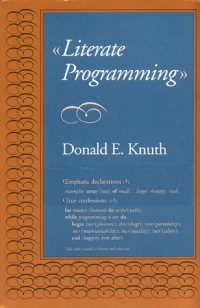
\includegraphics{inclusions/literate_programming_book_cover_smaller.png}

\captionsetup[floatingfigure]{labelformat=empty}
\begin{floatingfigure}[l]{0.22\textwidth}
\centering
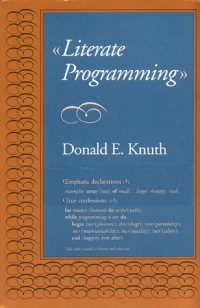
\includegraphics[width=0.18\textwidth]{inclusions/literate_programming_book_cover_smaller.png}
%\caption{~~~IMCAPTION~~~}
%\label{fig:2910X0}
\end{floatingfigure}Knuth applied Literate Programming to his \(\TeX\) systems and produced
what many consider
\href{https://www.amazon.com/TeXbook-Donald-Knuth/dp/0201134489\#customerReviews}{enduring
masterpieces} of program documentation.

\texttt{jodliterate} is certainly
\href{https://www.youtube.com/watch?v=o5FT3IGXtAk}{not worthy} of
\(\TeX\) level accolades but with a little work it's possible to produce
fine documents. This \href{https://github.com/martin-saurer/jkernel}{J
kernel notebook} outlines how you can install and use
\texttt{jodliterate}. \href{https://jupyter.org/}{Jupyter} notebooks are
typically executed but to accommodate J users that do hot have Jupyter
this notebook is also available on GitHub as a
\href{https://github.com/bakerjd99/jacks/blob/master/jodliterate/UsingJodliterate.pdf}{static
PDF document}.

    \hypertarget{notebook-preliminaries}{%
\paragraph{Notebook Preliminaries}\label{notebook-preliminaries}}

    \begin{tcolorbox}[breakable, size=fbox, boxrule=1pt, pad at break*=1mm,colback=cellbackground, colframe=cellborder]
\prompt{In}{incolor}{1}{\boxspacing}
\begin{Verbatim}[commandchars=\\\{\}]
\PY{c+c1}{NB. show J kernel version}
\PY{l+m+mi}{9}\PY{o}{!}\PY{o}{:}\PY{l+m+mi}{14} \PY{l+s}{\PYZsq{}}\PY{l+s}{\PYZsq{}}
\end{Verbatim}
\end{tcolorbox}

    \begin{Verbatim}[commandchars=\\\{\}]
j901/j64avx/windows/release-e/commercial/www.jsoftware.com/2020-01-29T11:15:50
    \end{Verbatim}

    \begin{tcolorbox}[breakable, size=fbox, boxrule=1pt, pad at break*=1mm,colback=cellbackground, colframe=cellborder]
\prompt{In}{incolor}{2}{\boxspacing}
\begin{Verbatim}[commandchars=\\\{\}]
\PY{c+c1}{NB. load JOD in a clear base locale}
\PY{n+nv}{load} \PY{l+s}{\PYZsq{}}\PY{l+s}{g}\PY{l+s}{e}\PY{l+s}{n}\PY{l+s}{e}\PY{l+s}{r}\PY{l+s}{a}\PY{l+s}{l}\PY{l+s}{/}\PY{l+s}{j}\PY{l+s}{o}\PY{l+s}{d}\PY{l+s}{\PYZsq{}} \PY{o}{[} \PY{n+nv}{clear} \PY{l+s}{\PYZsq{}}\PY{l+s}{\PYZsq{}}

\PY{c+c1}{NB. The distributed JOD profile automatically RESETME\PYZsq{}s.}
\PY{c+c1}{NB. To safely use dictionaries with many J tasks they must}
\PY{c+c1}{NB. be READONLY. To prevent opening the same put dictionary}
\PY{c+c1}{NB. READWRITE comment out (dpset) and restart this notebook.}
\PY{n+nv}{dpset} \PY{l+s}{\PYZsq{}}\PY{l+s}{R}\PY{l+s}{E}\PY{l+s}{S}\PY{l+s}{E}\PY{l+s}{T}\PY{l+s}{M}\PY{l+s}{E}\PY{l+s}{\PYZsq{}}

\PY{c+c1}{NB. Converting Jupyter notebooks to LaTeX is }
\PY{c+c1}{NB. simplified by ASCII box characters.}
\PY{n+nv}{portchars} \PY{l+s}{\PYZsq{}}\PY{l+s}{\PYZsq{}}

\PY{c+c1}{NB. Verb to show large boxed displays in}
\PY{c+c1}{NB. the notebook without ugly wrapping.}
\PY{n+nv}{sbx\PYZus{}ijod\PYZus{}}\PY{o}{=:} \PY{l+s}{\PYZsq{}}\PY{l+s}{ }\PY{l+s}{.}\PY{l+s}{.}\PY{l+s}{.}\PY{l+s}{ }\PY{l+s}{\PYZsq{}} \PY{o}{,}\PY{o}{\PYZdq{}}\PY{l+m+mi}{1}\PY{o}{\PYZti{}} \PY{l+m+mi}{75}\PY{o}{\PYZam{}}\PY{o}{\PYZob{}}\PY{o}{.}\PY{o}{\PYZdq{}}\PY{l+m+mi}{1}\PY{o}{@}\PY{o}{\PYZdq{}}\PY{o}{:}
\end{Verbatim}
\end{tcolorbox}

    \hypertarget{installing-jodliterate}{%
\paragraph{Installing jodliterate}\label{installing-jodliterate}}

To use \texttt{jodliterate} you need to:

\begin{enumerate}
\def\labelenumi{\arabic{enumi}.}
\tightlist
\item
  Install a current version of J.
\item
  Install the J addons JOD, JODSOURCE, and JODDOCUMENT.
\item
  Build the JOD development dictionaries from JODSOURCE.
\item
  Install a current version of \href{https://pandoc.org/}{pandoc}.
\item
  Install a current version of \(\TeX\) and \(\LaTeX\).
\item
  Make the \texttt{jodliterate} J script.
\item
  Run \texttt{jodliterate} on a JOD \emph{group} with pandoc compatible
  document fragments.
\item
  Compile the files of the previous step to produce a PDF
\end{enumerate}

When presented with long lists of program prerequisites my impulse is to
\emph{run!} Life is too short for configuration wars. Everything should
be easy. Installing \texttt{jodliterate} requires more work than phone
apps but compared to
\href{https://www.cio.com/article/2429865/enterprise-resource-planning-10-famous-erp-disasters-dustups-and-disappointments.html}{enterprise
installations} setting up \texttt{jodliterate} is trivial. We'll go
through it step by step.

    \hypertarget{step-1-install-a-current-version-of-j}{%
\paragraph{Step 1: Install a current version of
J}\label{step-1-install-a-current-version-of-j}}

J is freely available at
\href{https://www.jsoftware.com}{jsoftware.com}. J installation
instructions can be found on the
\href{https://code.jsoftware.com/wiki/Main_Page}{J Wiki} on
\href{https://code.jsoftware.com/wiki/System/Installation}{this page}.

Follow the appropriate instructions for your OS.

\textbf{Note:} JOD runs on Windows, Linux, and MacOS versions of J,
hence these are the only platforms that currently support
\texttt{jodliterate}.

    \hypertarget{step-2-install-the-j-addons-jod-jodsource-and-joddocument}{%
\paragraph{Step 2: Install the J addons JOD, JODSOURCE and
JODDOCUMENT}\label{step-2-install-the-j-addons-jod-jodsource-and-joddocument}}

After installing J install the J addons. J addons are installed with the
J package manager \href{https://code.jsoftware.com/wiki/Pacman}{pacman}.
Pacman has three
\href{https://en.wikipedia.org/wiki/Integrated_development_environment}{IDE}
flavors: a command-line flavor and two GUI flavors. The GUI flavors
depend on \href{https://code.jsoftware.com/wiki/Guides/Qt_IDE}{JQT} or
\href{https://code.jsoftware.com/wiki/Guides/JHS/Server}{JHS}. The GUI
flavors of pacman are only available on some versions of J whereas the
command line version is part of the base J install and is available on
all platforms.

\textbf{\emph{I install all the addons. I recommend that you do the
same.}}

JOD depends on some J modules like \texttt{jfiles}, \texttt{regex}, and
\texttt{task} that are sometimes distributed as addons. If you install
all addons JOD's modules and dependents are both installed.

    \hypertarget{installing-addons-with-command-line-pacman}{%
\paragraph{Installing addons with command line
pacman}\label{installing-addons-with-command-line-pacman}}

Start J and do:

    \begin{tcolorbox}[breakable, size=fbox, boxrule=1pt, pad at break*=1mm,colback=cellbackground, colframe=cellborder]
\prompt{In}{incolor}{3}{\boxspacing}
\begin{Verbatim}[commandchars=\\\{\}]
\PY{c+c1}{NB. install J addons with command\PYZhy{}line pacman}

\PY{n+nv}{load} \PY{l+s}{\PYZsq{}}\PY{l+s}{p}\PY{l+s}{a}\PY{l+s}{c}\PY{l+s}{m}\PY{l+s}{a}\PY{l+s}{n}\PY{l+s}{\PYZsq{}}    \PY{c+c1}{NB. load pacman jpkg services}
\end{Verbatim}
\end{tcolorbox}

    \begin{tcolorbox}[breakable, size=fbox, boxrule=1pt, pad at break*=1mm,colback=cellbackground, colframe=cellborder]
\prompt{In}{incolor}{4}{\boxspacing}
\begin{Verbatim}[commandchars=\\\{\}]
\PY{l+s}{\PYZsq{}}\PY{l+s}{h}\PY{l+s}{e}\PY{l+s}{l}\PY{l+s}{p}\PY{l+s}{\PYZsq{}} \PY{n+nv}{jpkg} \PY{l+s}{\PYZsq{}}\PY{l+s}{\PYZsq{}}   \PY{c+c1}{NB. what can you do for me?}
\end{Verbatim}
\end{tcolorbox}

    \begin{Verbatim}[commandchars=\\\{\}]
Valid options are:
 history, install, manifest, remove, reinstall, search,
 show, showinstalled, shownotinstalled, showupgrade,
 status, update, upgrade

https://code.jsoftware.com/wiki/JAL/Package\_Manager/jpkg

    \end{Verbatim}

    \begin{tcolorbox}[breakable, size=fbox, boxrule=1pt, pad at break*=1mm,colback=cellbackground, colframe=cellborder]
\prompt{In}{incolor}{5}{\boxspacing}
\begin{Verbatim}[commandchars=\\\{\}]
\PY{c+c1}{NB. install all addons}
\PY{c+c1}{NB. see https://code.jsoftware.com/wiki/Pacman}

\PY{c+c1}{NB. uncomment next line if addons not installed}
\PY{c+c1}{NB. \PYZsq{}install\PYZsq{} jpkg \PYZsq{}*\PYZsq{}  NB.}
\end{Verbatim}
\end{tcolorbox}

    \begin{tcolorbox}[breakable, size=fbox, boxrule=1pt, pad at break*=1mm,colback=cellbackground, colframe=cellborder]
\prompt{In}{incolor}{6}{\boxspacing}
\begin{Verbatim}[commandchars=\\\{\}]
\PY{l+m+mi}{3} \PY{o}{\PYZob{}}\PY{o}{.} \PY{l+s}{\PYZsq{}}\PY{l+s}{s}\PY{l+s}{h}\PY{l+s}{o}\PY{l+s}{w}\PY{l+s}{i}\PY{l+s}{n}\PY{l+s}{s}\PY{l+s}{t}\PY{l+s}{a}\PY{l+s}{l}\PY{l+s}{l}\PY{l+s}{e}\PY{l+s}{d}\PY{l+s}{\PYZsq{}} \PY{n+nv}{jpkg} \PY{l+s}{\PYZsq{}}\PY{l+s}{\PYZsq{}} \PY{c+c1}{NB. first few installed addons}
\end{Verbatim}
\end{tcolorbox}

    \begin{Verbatim}[commandchars=\\\{\}]
+---------+------+------+-----------------------------+
|api/expat|1.0.11|1.0.11|libexpat                     |
+---------+------+------+-----------------------------+
|api/gles |1.0.31|1.0.31|Modern OpenGL API            |
+---------+------+------+-----------------------------+
|api/java |1.0.2 |1.0.2 |api: Java to J shared library|
+---------+------+------+-----------------------------+
    \end{Verbatim}

    \begin{tcolorbox}[breakable, size=fbox, boxrule=1pt, pad at break*=1mm,colback=cellbackground, colframe=cellborder]
\prompt{In}{incolor}{7}{\boxspacing}
\begin{Verbatim}[commandchars=\\\{\}]
\PY{l+s}{\PYZsq{}}\PY{l+s}{s}\PY{l+s}{h}\PY{l+s}{o}\PY{l+s}{w}\PY{l+s}{u}\PY{l+s}{p}\PY{l+s}{g}\PY{l+s}{r}\PY{l+s}{a}\PY{l+s}{d}\PY{l+s}{e}\PY{l+s}{\PYZsq{}} \PY{n+nv}{jpkg} \PY{l+s}{\PYZsq{}}\PY{l+s}{\PYZsq{}}  \PY{c+c1}{NB. list addon updates}
\end{Verbatim}
\end{tcolorbox}

    \hypertarget{installing-addons-with-jqt-gui-pacman}{%
\paragraph{Installing addons with JQT GUI
pacman}\label{installing-addons-with-jqt-gui-pacman}}

    I mostly use the Windows JQT version of pacman to install and maintain J
addons. You can find pacman on the tools menu.

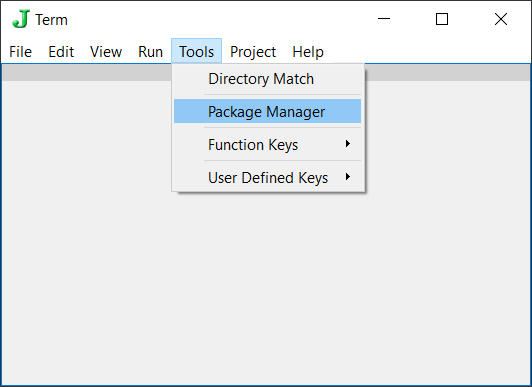
\includegraphics{inclusions/jqt_pacman_menu-1.png}

pacman shows all available addons and provides tools for installing,
updating, and removing them.

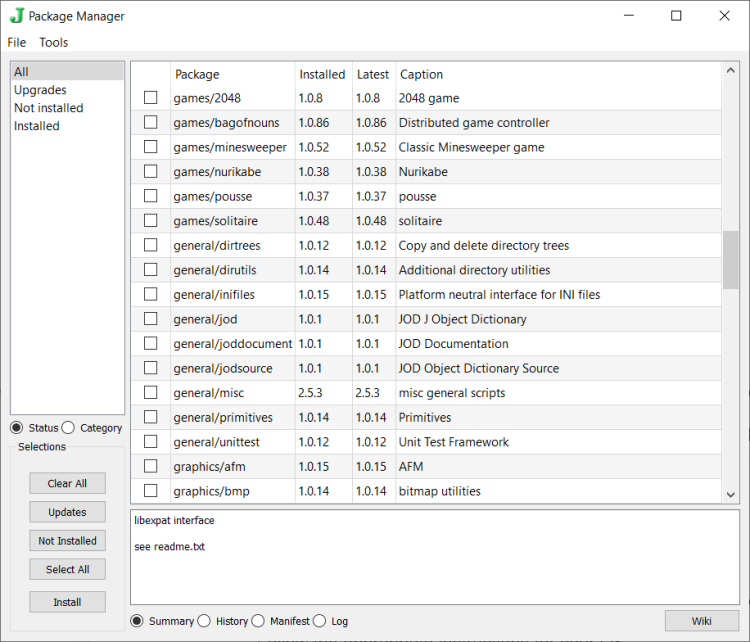
\includegraphics{inclusions/jqt_pacman.png}

The GUI version is easy to use. Press the \texttt{Select\ All} button
and then press the \texttt{Install} button to install all the addons. To
update addons select the \texttt{Upgrades} menu and select the addons
you want to update.

    \hypertarget{step-3-build-the-jod-development-dictionaries-from-jodsource}{%
\paragraph{Step 3: Build the JOD development dictionaries from
JODSOURCE}\label{step-3-build-the-jod-development-dictionaries-from-jodsource}}

JOD source code is distributed in the form of
\href{https://github.com/bakerjd99/joddumps}{JOD dictionary dumps}.
Dictionary dumps are large J scripts that serialize JOD dictionaries.
Dumps contain everything stored in dictionaries. You will find source
code, binary data, test scripts, documentation, build macros, and more
in typical JOD dictionaries.

\texttt{jodliterate} is stored as a JOD dictionary group. A dictionary
group is simply a collection of J words with optional \emph{header} and
\emph{post-processor} scripts. JOD generates J scripts from groups.
Before we can \emph{make} \texttt{jodliterate} we must load the JOD
development dictionaries. The JODSOURCE addon includes a J script that
\href{https://github.com/bakerjd99/jod/blob/master/jodsource/jodsourcesetup.ijs}{loads
development dictionaries}.

Again, start J and do:

    \begin{tcolorbox}[breakable, size=fbox, boxrule=1pt, pad at break*=1mm,colback=cellbackground, colframe=cellborder]
\prompt{In}{incolor}{8}{\boxspacing}
\begin{Verbatim}[commandchars=\\\{\}]
\PY{n+nv}{require} \PY{l+s}{\PYZsq{}}\PY{l+s}{g}\PY{l+s}{e}\PY{l+s}{n}\PY{l+s}{e}\PY{l+s}{r}\PY{l+s}{a}\PY{l+s}{l}\PY{l+s}{/}\PY{l+s}{j}\PY{l+s}{o}\PY{l+s}{d}\PY{l+s}{\PYZsq{}}
\end{Verbatim}
\end{tcolorbox}

    \begin{tcolorbox}[breakable, size=fbox, boxrule=1pt, pad at break*=1mm,colback=cellbackground, colframe=cellborder]
\prompt{In}{incolor}{9}{\boxspacing}
\begin{Verbatim}[commandchars=\\\{\}]
\PY{c+c1}{NB. set a JODroot user folder }
\PY{c+c1}{NB. if not set /jod/ is the default}

\PY{c+c1}{NB. use paths for your OS}
\PY{n+nv}{UserFolders\PYZus{}j\PYZus{}}\PY{o}{=:} \PY{n+nv}{UserFolders\PYZus{}j\PYZus{}} \PY{o}{,} \PY{l+s}{\PYZsq{}}\PY{l+s}{J}\PY{l+s}{O}\PY{l+s}{D}\PY{l+s}{r}\PY{l+s}{o}\PY{l+s}{o}\PY{l+s}{t}\PY{l+s}{\PYZsq{}}\PY{o}{;}\PY{l+s}{\PYZsq{}}\PY{l+s}{c}\PY{l+s}{:}\PY{l+s}{/}\PY{l+s}{t}\PY{l+s}{e}\PY{l+s}{m}\PY{l+s}{p}\PY{l+s}{\PYZsq{}}

\PY{c+c1}{NB. show added folder}
\PY{n+nv}{UserFolders\PYZus{}j\PYZus{}} \PY{o}{\PYZob{}}\PY{o}{\PYZti{}} \PY{p}{(}\PY{l+m+mi}{0} \PY{o}{\PYZob{}}\PY{o}{\PYZdq{}}\PY{l+m+mi}{1} \PY{n+nv}{UserFolders\PYZus{}j\PYZus{}}\PY{p}{)} \PY{n+nv}{i}\PY{o}{.} \PY{o}{\PYZlt{}}\PY{l+s}{\PYZsq{}}\PY{l+s}{J}\PY{l+s}{O}\PY{l+s}{D}\PY{l+s}{r}\PY{l+s}{o}\PY{l+s}{o}\PY{l+s}{t}\PY{l+s}{\PYZsq{}}
\end{Verbatim}
\end{tcolorbox}

    \begin{Verbatim}[commandchars=\\\{\}]
+-------+-------+
|JODroot|c:/temp|
+-------+-------+
    \end{Verbatim}

    \begin{tcolorbox}[breakable, size=fbox, boxrule=1pt, pad at break*=1mm,colback=cellbackground, colframe=cellborder]
\prompt{In}{incolor}{10}{\boxspacing}
\begin{Verbatim}[commandchars=\\\{\}]
\PY{c+c1}{NB. load JOD developement dictionaries}
\PY{n+nv}{load\PYZus{}dev\PYZus{}tmp}\PY{o}{=:} \PY{n+nf}{3 : 0}
\PY{n+nl}{if.} \PY{o}{+}\PY{o}{.}\PY{o}{/} \PY{p}{(}\PY{o}{;}\PY{o}{:}\PY{l+s}{\PYZsq{}}\PY{l+s}{j}\PY{l+s}{o}\PY{l+s}{d}\PY{l+s}{d}\PY{l+s}{e}\PY{l+s}{v}\PY{l+s}{ }\PY{l+s}{j}\PY{l+s}{o}\PY{l+s}{d}\PY{l+s}{ }\PY{l+s}{u}\PY{l+s}{t}\PY{l+s}{i}\PY{l+s}{l}\PY{l+s}{s}\PY{l+s}{\PYZsq{}}\PY{p}{)} \PY{n+nv}{e}\PY{o}{.} \PY{n+nv}{od} \PY{l+s}{\PYZsq{}}\PY{l+s}{\PYZsq{}} \PY{n+nl}{do.}
  \PY{l+s}{\PYZsq{}}\PY{l+s}{d}\PY{l+s}{e}\PY{l+s}{v}\PY{l+s}{ }\PY{l+s}{d}\PY{l+s}{i}\PY{l+s}{c}\PY{l+s}{t}\PY{l+s}{i}\PY{l+s}{o}\PY{l+s}{n}\PY{l+s}{a}\PY{l+s}{r}\PY{l+s}{i}\PY{l+s}{e}\PY{l+s}{s}\PY{l+s}{ }\PY{l+s}{e}\PY{l+s}{x}\PY{l+s}{i}\PY{l+s}{s}\PY{l+s}{t}\PY{l+s}{\PYZsq{}}
\PY{n+nl}{else.}
  \PY{l+m+mi}{0}\PY{o}{!}\PY{o}{:}\PY{l+m+mi}{0}\PY{o}{\PYZlt{}}\PY{n+nv}{jpath}\PY{l+s}{\PYZsq{}}\PY{l+s}{\PYZti{}}\PY{l+s}{a}\PY{l+s}{d}\PY{l+s}{d}\PY{l+s}{o}\PY{l+s}{n}\PY{l+s}{s}\PY{l+s}{/}\PY{l+s}{g}\PY{l+s}{e}\PY{l+s}{n}\PY{l+s}{e}\PY{l+s}{r}\PY{l+s}{a}\PY{l+s}{l}\PY{l+s}{/}\PY{l+s}{j}\PY{l+s}{o}\PY{l+s}{d}\PY{l+s}{s}\PY{l+s}{o}\PY{l+s}{u}\PY{l+s}{r}\PY{l+s}{c}\PY{l+s}{e}\PY{l+s}{/}\PY{l+s}{j}\PY{l+s}{o}\PY{l+s}{d}\PY{l+s}{s}\PY{l+s}{o}\PY{l+s}{u}\PY{l+s}{r}\PY{l+s}{c}\PY{l+s}{e}\PY{l+s}{s}\PY{l+s}{e}\PY{l+s}{t}\PY{l+s}{u}\PY{l+s}{p}\PY{l+s}{.}\PY{l+s}{i}\PY{l+s}{j}\PY{l+s}{s}\PY{l+s}{\PYZsq{}}
\PY{n+nl}{end.}
\PY{n+nl}{)}

\PY{n+nv}{load\PYZus{}dev\PYZus{}tmp} \PY{l+m+mi}{0}
\end{Verbatim}
\end{tcolorbox}

    \begin{Verbatim}[commandchars=\\\{\}]
dev dictionaries exist
    \end{Verbatim}

    \begin{tcolorbox}[breakable, size=fbox, boxrule=1pt, pad at break*=1mm,colback=cellbackground, colframe=cellborder]
\prompt{In}{incolor}{11}{\boxspacing}
\begin{Verbatim}[commandchars=\\\{\}]
\PY{c+c1}{NB. joddev, jod, utils should exist}

\PY{n+nv}{erase} \PY{l+s}{\PYZsq{}}\PY{l+s}{l}\PY{l+s}{o}\PY{l+s}{a}\PY{l+s}{d}\PY{l+s}{\PYZus{}}\PY{l+s}{d}\PY{l+s}{e}\PY{l+s}{v}\PY{l+s}{\PYZus{}}\PY{l+s}{t}\PY{l+s}{m}\PY{l+s}{p}\PY{l+s}{\PYZsq{}}
\PY{p}{(}\PY{o}{;}\PY{o}{:}\PY{l+s}{\PYZsq{}}\PY{l+s}{j}\PY{l+s}{o}\PY{l+s}{d}\PY{l+s}{d}\PY{l+s}{e}\PY{l+s}{v}\PY{l+s}{ }\PY{l+s}{j}\PY{l+s}{o}\PY{l+s}{d}\PY{l+s}{ }\PY{l+s}{u}\PY{l+s}{t}\PY{l+s}{i}\PY{l+s}{l}\PY{l+s}{s}\PY{l+s}{\PYZsq{}}\PY{p}{)} \PY{n+nv}{e}\PY{o}{.} \PY{n+nv}{od} \PY{l+s}{\PYZsq{}}\PY{l+s}{\PYZsq{}}
\end{Verbatim}
\end{tcolorbox}

    \begin{Verbatim}[commandchars=\\\{\}]
1 1 1
    \end{Verbatim}

    \hypertarget{step-4-install-a-current-version-of-pandoc}{%
\paragraph{Step 4: Install a current version of
pandoc}\label{step-4-install-a-current-version-of-pandoc}}

\href{https://pandoc.org/}{pandoc} is easily one of the most useful
markup utilities on the
\href{https://www.urbandictionary.com/define.php?term=intertubes}{intertubes}.
If you routinely deal with markup formats like markdown, XML,
\(\LaTeX\), json and you aren't using pandoc you are working too hard.

Be lazy! \href{https://pandoc.org/installing.html}{Install pandoc}.

\texttt{jodliterate} uses the \texttt{task} addon to \emph{shell out} to
pandoc. Versions of pandoc after \texttt{2.9.1.1} support J syntax
high-lighting.

    \begin{tcolorbox}[breakable, size=fbox, boxrule=1pt, pad at break*=1mm,colback=cellbackground, colframe=cellborder]
\prompt{In}{incolor}{12}{\boxspacing}
\begin{Verbatim}[commandchars=\\\{\}]
\PY{c+c1}{NB. show pandoc version from J \PYZhy{} make sure you are running }
\PY{c+c1}{NB. a recent version of pandoc. There may be different}
\PY{c+c1}{NB. versions in many locations on various systems.}

\PY{n+nv}{ppath}\PY{o}{=:} \PY{l+s}{\PYZsq{}}\PY{l+s}{\PYZdq{}}\PY{l+s}{C}\PY{l+s}{:}\PY{l+s}{\PYZbs{}}\PY{l+s}{P}\PY{l+s}{r}\PY{l+s}{o}\PY{l+s}{g}\PY{l+s}{r}\PY{l+s}{a}\PY{l+s}{m}\PY{l+s}{ }\PY{l+s}{F}\PY{l+s}{i}\PY{l+s}{l}\PY{l+s}{e}\PY{l+s}{s}\PY{l+s}{\PYZbs{}}\PY{l+s}{P}\PY{l+s}{a}\PY{l+s}{n}\PY{l+s}{d}\PY{l+s}{o}\PY{l+s}{c}\PY{l+s}{\PYZbs{}}\PY{l+s}{p}\PY{l+s}{a}\PY{l+s}{n}\PY{l+s}{d}\PY{l+s}{o}\PY{l+s}{c}\PY{l+s}{\PYZdq{}}\PY{l+s}{\PYZsq{}}
\PY{n+nv}{THISPANDOC\PYZus{}ajodliterate\PYZus{}}\PY{o}{=:} \PY{n+nv}{ppath}
\PY{n+nv}{shell} \PY{n+nv}{THISPANDOC\PYZus{}ajodliterate\PYZus{}}\PY{o}{,}\PY{l+s}{\PYZsq{}}\PY{l+s}{ }\PY{l+s}{\PYZhy{}}\PY{l+s}{\PYZhy{}}\PY{l+s}{v}\PY{l+s}{e}\PY{l+s}{r}\PY{l+s}{s}\PY{l+s}{i}\PY{l+s}{o}\PY{l+s}{n}\PY{l+s}{\PYZsq{}}
\end{Verbatim}
\end{tcolorbox}

    \begin{Verbatim}[commandchars=\\\{\}]
pandoc 2.9.1.1
Compiled with pandoc-types 1.20, texmath 0.12, skylighting 0.8.3
Default user data directory: C:\textbackslash{}Users\textbackslash{}john\textbackslash{}AppData\textbackslash{}Roaming\textbackslash{}pandoc
Copyright (C) 2006-2019 John MacFarlane
Web:  https://pandoc.org
This is free software; see the source for copying conditions.
There is no warranty, not even for merchantability or fitness
for a particular purpose.

    \end{Verbatim}

    \begin{tcolorbox}[breakable, size=fbox, boxrule=1pt, pad at break*=1mm,colback=cellbackground, colframe=cellborder]
\prompt{In}{incolor}{13}{\boxspacing}
\begin{Verbatim}[commandchars=\\\{\}]
\PY{c+c1}{NB. make sure your version of pandoc }
\PY{c+c1}{NB. supports J syntax\PYZhy{}highlighting}

\PY{c+c1}{NB. appends line feed character if necessary}
\PY{n+nv}{tlf}\PY{o}{=:}\PY{o}{]} \PY{o}{,} \PY{p}{(}\PY{p}{(}\PY{l+m+mi}{10}\PY{o}{\PYZob{}}\PY{n+nv}{a}\PY{o}{.}\PY{p}{)}\PY{o}{\PYZdq{}}\PY{l+m}{\PYZus{}} \PY{o}{=} \PY{o}{\PYZob{}}\PY{o}{:}\PY{p}{)} \PY{o}{\PYZcb{}}\PY{o}{.} \PY{p}{(}\PY{l+m+mi}{10}\PY{o}{\PYZob{}}\PY{n+nv}{a}\PY{o}{.}\PY{p}{)}\PY{o}{\PYZdq{}}\PY{l+m}{\PYZus{}}

\PY{c+c1}{NB. J is on the supported languages list}
\PY{n+nv}{pcmd}\PY{o}{=:} \PY{n+nv}{THISPANDOC\PYZus{}ajodliterate\PYZus{}}\PY{o}{,}\PY{l+s}{\PYZsq{}}\PY{l+s}{ }\PY{l+s}{\PYZhy{}}\PY{l+s}{\PYZhy{}}\PY{l+s}{l}\PY{l+s}{i}\PY{l+s}{s}\PY{l+s}{t}\PY{l+s}{\PYZhy{}}\PY{l+s}{h}\PY{l+s}{i}\PY{l+s}{g}\PY{l+s}{h}\PY{l+s}{l}\PY{l+s}{i}\PY{l+s}{g}\PY{l+s}{h}\PY{l+s}{t}\PY{l+s}{\PYZhy{}}\PY{l+s}{l}\PY{l+s}{a}\PY{l+s}{n}\PY{l+s}{g}\PY{l+s}{u}\PY{l+s}{a}\PY{l+s}{g}\PY{l+s}{e}\PY{l+s}{s}\PY{l+s}{\PYZsq{}}
\PY{p}{(}\PY{o}{\PYZlt{}}\PY{o}{;}\PY{o}{.}\PY{l+m+mi}{\PYZus{}2} \PY{n+nv}{tlf} \PY{p}{(}\PY{n+nv}{shell} \PY{n+nv}{pcmd}\PY{p}{)} \PY{o}{\PYZhy{}}\PY{o}{.} \PY{n+nv}{CR}\PY{p}{)} \PY{n+nv}{e}\PY{o}{.}\PY{o}{\PYZti{}} \PY{o}{\PYZlt{}}\PY{o}{,}\PY{l+s}{\PYZsq{}}\PY{l+s}{j}\PY{l+s}{\PYZsq{}}
\end{Verbatim}
\end{tcolorbox}

    \begin{Verbatim}[commandchars=\\\{\}]
1
    \end{Verbatim}

    \hypertarget{step-5-install-a-current-version-of-latex}{%
\paragraph{Step 5: Install a current version of
LaTeX}\label{step-5-install-a-current-version-of-latex}}

\texttt{jodliterate} uses \(\LaTeX\) to compile PDF documents. When
\texttt{setjodliterate} runs it sets an output directory and writes a
\(\LaTeX\) preamble file \texttt{JODLiteratePreamble.tex} to it. It's a
good idea to review this file to get an idea of the \(\LaTeX\) packages
\texttt{jodliterate} uses. It's possible that some of these packages are
not in your \(\LaTeX\) distribution and will have to be installed.

To ease the burden of \(\LaTeX\) package maintenance I use freely
available \(\TeX\) versions that automatically install missing packages.

\begin{enumerate}
\def\labelenumi{\arabic{enumi}.}
\tightlist
\item
  On Windows I use \href{https://miktex.org/}{MiKTeX}
\item
  On other platforms I use
  \href{https://en.wikipedia.org/wiki/TeX_Live}{TeXLive}
\end{enumerate}

If your system automatically installs packages the first time you
compile \texttt{jodliterate} output it may fetch missing packages from
The Comprehensive \(\TeX\) Archive Network
\href{https://www.ctan.org/}{(CTAN)}. If new packages are installed
reprocess your files a few times to insure all the required packages are
downloaded and installed.

    \hypertarget{step-6-make-the-jodliterate-j-script}{%
\paragraph{Step: 6 Make the jodliterate J
script}\label{step-6-make-the-jodliterate-j-script}}

Once the JOD development dictionaries are built (Step 3) making
\texttt{jodliterate} is easy. Start J and do:

    \begin{tcolorbox}[breakable, size=fbox, boxrule=1pt, pad at break*=1mm,colback=cellbackground, colframe=cellborder]
\prompt{In}{incolor}{14}{\boxspacing}
\begin{Verbatim}[commandchars=\\\{\}]
\PY{n+nv}{require} \PY{l+s}{\PYZsq{}}\PY{l+s}{g}\PY{l+s}{e}\PY{l+s}{n}\PY{l+s}{e}\PY{l+s}{r}\PY{l+s}{a}\PY{l+s}{l}\PY{l+s}{/}\PY{l+s}{j}\PY{l+s}{o}\PY{l+s}{d}\PY{l+s}{\PYZsq{}}

\PY{c+c1}{NB. open dictionaries}
\PY{n+nv}{od} \PY{o}{;}\PY{o}{:}\PY{l+s}{\PYZsq{}}\PY{l+s}{j}\PY{l+s}{o}\PY{l+s}{d}\PY{l+s}{d}\PY{l+s}{e}\PY{l+s}{v}\PY{l+s}{ }\PY{l+s}{j}\PY{l+s}{o}\PY{l+s}{d}\PY{l+s}{ }\PY{l+s}{u}\PY{l+s}{t}\PY{l+s}{i}\PY{l+s}{l}\PY{l+s}{s}\PY{l+s}{\PYZsq{}} \PY{o}{[} \PY{l+m+mi}{3} \PY{n+nv}{od} \PY{l+s}{\PYZsq{}}\PY{l+s}{\PYZsq{}}
\end{Verbatim}
\end{tcolorbox}

    \begin{Verbatim}[commandchars=\\\{\}]
+-+--------------------+------+---+-----+
|1|opened (rw/ro/ro) ->|joddev|jod|utils|
+-+--------------------+------+---+-----+
    \end{Verbatim}

    \begin{tcolorbox}[breakable, size=fbox, boxrule=1pt, pad at break*=1mm,colback=cellbackground, colframe=cellborder]
\prompt{In}{incolor}{15}{\boxspacing}
\begin{Verbatim}[commandchars=\\\{\}]
\PY{c+c1}{NB. generate jodliterate}
\PY{n+nv}{sbx} \PY{n+nv}{mls} \PY{l+s}{\PYZsq{}}\PY{l+s}{j}\PY{l+s}{o}\PY{l+s}{d}\PY{l+s}{l}\PY{l+s}{i}\PY{l+s}{t}\PY{l+s}{e}\PY{l+s}{r}\PY{l+s}{a}\PY{l+s}{t}\PY{l+s}{e}\PY{l+s}{\PYZsq{}}
\end{Verbatim}
\end{tcolorbox}

    \begin{Verbatim}[commandchars=\\\{\}]
+-+--------------------+------------------------------------+               {\ldots}
|1|load script saved ->|c:/jod/joddev/script/jodliterate.ijs|               {\ldots}
+-+--------------------+------------------------------------+               {\ldots}
    \end{Verbatim}

    \texttt{mls} creates a standard J load script. Once generated this
script can be loaded with the standard J \texttt{load} utility. You can
test this by restarting J without JOD and loading \texttt{jodliterate}.

    \begin{tcolorbox}[breakable, size=fbox, boxrule=1pt, pad at break*=1mm,colback=cellbackground, colframe=cellborder]
\prompt{In}{incolor}{16}{\boxspacing}
\begin{Verbatim}[commandchars=\\\{\}]
\PY{c+c1}{NB. load generated script}
\PY{n+nv}{load} \PY{l+s}{\PYZsq{}}\PY{l+s}{j}\PY{l+s}{o}\PY{l+s}{d}\PY{l+s}{l}\PY{l+s}{i}\PY{l+s}{t}\PY{l+s}{e}\PY{l+s}{r}\PY{l+s}{a}\PY{l+s}{t}\PY{l+s}{e}\PY{l+s}{\PYZsq{}}
\end{Verbatim}
\end{tcolorbox}

    \begin{Verbatim}[commandchars=\\\{\}]
NB. (jodliterate) interface word(s):
NB. --------------------------------
NB. THISPANDOC      NB. full pandoc path - use (pandoc) if on shell path
NB. grplit          NB. make latex for group (y)
NB. ifacesection    NB. interface section summary string
NB. ifc             NB. format interface comment text
NB. setjodliterate  NB. prepare LaTeX processing - sets out directory writes
preamble

NOTE: adjust pandoc path if version (pandoc 2.9.1.1) is not >= 2.9.1.1
    \end{Verbatim}

    \hypertarget{step-7-run-jodliterate-on-a-jod-group-with-pandoc-compatible-document-fragments}{%
\paragraph{Step 7: Run jodliterate on a JOD group with pandoc compatible
document
fragments}\label{step-7-run-jodliterate-on-a-jod-group-with-pandoc-compatible-document-fragments}}

This sounds a lot worse than it is. There is a group in \texttt{utils}
called \texttt{sunmoon} that has an interesting \emph{pandoc compatible
document fragment}.

Start J and do:

    \begin{tcolorbox}[breakable, size=fbox, boxrule=1pt, pad at break*=1mm,colback=cellbackground, colframe=cellborder]
\prompt{In}{incolor}{17}{\boxspacing}
\begin{Verbatim}[commandchars=\\\{\}]
\PY{n+nv}{require} \PY{l+s}{\PYZsq{}}\PY{l+s}{g}\PY{l+s}{e}\PY{l+s}{n}\PY{l+s}{e}\PY{l+s}{r}\PY{l+s}{a}\PY{l+s}{l}\PY{l+s}{/}\PY{l+s}{j}\PY{l+s}{o}\PY{l+s}{d}\PY{l+s}{\PYZsq{}}

\PY{n+nv}{od} \PY{l+s}{\PYZsq{}}\PY{l+s}{u}\PY{l+s}{t}\PY{l+s}{i}\PY{l+s}{l}\PY{l+s}{s}\PY{l+s}{\PYZsq{}} \PY{o}{[} \PY{l+m+mi}{3} \PY{n+nv}{od} \PY{l+s}{\PYZsq{}}\PY{l+s}{\PYZsq{}}
\end{Verbatim}
\end{tcolorbox}

    \begin{Verbatim}[commandchars=\\\{\}]
+-+--------------+-----+
|1|opened (ro) ->|utils|
+-+--------------+-----+
    \end{Verbatim}

    \begin{tcolorbox}[breakable, size=fbox, boxrule=1pt, pad at break*=1mm,colback=cellbackground, colframe=cellborder]
\prompt{In}{incolor}{18}{\boxspacing}
\begin{Verbatim}[commandchars=\\\{\}]
\PY{c+c1}{NB. display short explanations for (sunmoon) words}
\PY{n+nv}{sbx} \PY{n+nv}{hlpnl} \PY{o}{\PYZcb{}}\PY{o}{.} \PY{n+nv}{grp} \PY{l+s}{\PYZsq{}}\PY{l+s}{s}\PY{l+s}{u}\PY{l+s}{n}\PY{l+s}{m}\PY{l+s}{o}\PY{l+s}{o}\PY{l+s}{n}\PY{l+s}{\PYZsq{}}
\end{Verbatim}
\end{tcolorbox}

    \begin{Verbatim}[commandchars=\\\{\}]
+-----------------+-------------------------------------------------------- {\ldots}
|IFACEWORDSsunmoon|interface words (IFACEWORDSsunmoon) group                {\ldots}
|NORISESET        |indicates sun never rises or sets in (sunriseset0) and ( {\ldots}
|ROOTWORDSsunmoon |root words (ROOTWORDSsunmoon) group                      {\ldots}
|arctan           |arc tangent                                              {\ldots}
|calmoons         |calendar dates of new and full moons                     {\ldots}
|cos              |cosine radians                                           {\ldots}
|fromjulian       |converts Julian day numbers to dates, converse (tojulian {\ldots}
|moons            |times of new and full moons for n calendar years         {\ldots}
|round            |round (y) to nearest (x) (e.g. 1000 round 12345)         {\ldots}
|sin              |sine radians                                             {\ldots}
|sunriseset0      |computes sun rise and set times - see group documentatio {\ldots}
|sunriseset1      |computes sun rise and set times - see group documentatio {\ldots}
|tabit            |promotes only atoms and lists to tables                  {\ldots}
|tan              |tan radians                                              {\ldots}
|today            |returns todays date                                      {\ldots}
|yeardates        |returns all valid dates for n calendar years             {\ldots}
+-----------------+-------------------------------------------------------- {\ldots}
    \end{Verbatim}

    \begin{tcolorbox}[breakable, size=fbox, boxrule=1pt, pad at break*=1mm,colback=cellbackground, colframe=cellborder]
\prompt{In}{incolor}{19}{\boxspacing}
\begin{Verbatim}[commandchars=\\\{\}]
\PY{c+c1}{NB. display part of the (sunmoon) group document header}
\PY{c+c1}{NB. this is pandoc compatible markdown \PYZhy{} note the LaTeX}
\PY{c+c1}{NB. commands \PYZhy{} pandoc allows markdown/LaTeX mixtures}
\PY{l+m+mi}{900} \PY{o}{\PYZob{}}\PY{o}{.} \PY{l+m+mi}{2} \PY{l+m+mi}{9} \PY{n+nv}{disp} \PY{l+s}{\PYZsq{}}\PY{l+s}{s}\PY{l+s}{u}\PY{l+s}{n}\PY{l+s}{m}\PY{l+s}{o}\PY{l+s}{o}\PY{l+s}{n}\PY{l+s}{\PYZsq{}}
\end{Verbatim}
\end{tcolorbox}

    \begin{Verbatim}[commandchars=\\\{\}]
`sunmoon` is a collection of basic astronomical algorithms
The key verbs are `moons`, `sunriseset0` and `sunriseset1.`
All of these verbs were derived from BASIC programs published
in *Sky \& Telescope* magazine in the 1990's. The rest of
the verbs in `sunmoon` are mostly date and trigonometric
utilities.

\textbackslash{}subsection\{\textbackslash{}texttt\{sunmoon\} Interface\}

\textasciitilde{}\textasciitilde{}\textasciitilde{}\textasciitilde{} \{ .j \}
  calmoons      NB. calendar dates of new and full moons
  moons         NB. times of new and full moons for n calendar years
  sunriseset0   NB. computes sun rise and set times - see group documentation
  sunriseset1   NB. computes sun rise and set times - see group documentation
\textasciitilde{}\textasciitilde{}\textasciitilde{}\textasciitilde{}

\textbackslash{}subsection\{\textbackslash{}textbf\textbackslash{}texttt\{sunriseset0\} \textbackslash{}textsl\{v--\} sunrise and sunset times\}

This  verb has been adapted from a BASIC program submitted by
Robin  G.  Stuart  *Sky \& Telescope's*  shortest  sunrise/set
program  cont
    \end{Verbatim}

    \begin{tcolorbox}[breakable, size=fbox, boxrule=1pt, pad at break*=1mm,colback=cellbackground, colframe=cellborder]
\prompt{In}{incolor}{20}{\boxspacing}
\begin{Verbatim}[commandchars=\\\{\}]
\PY{c+c1}{NB. run jodliterate on (sunmoon)}
\PY{n+nv}{require} \PY{l+s}{\PYZsq{}}\PY{l+s}{j}\PY{l+s}{o}\PY{l+s}{d}\PY{l+s}{l}\PY{l+s}{i}\PY{l+s}{t}\PY{l+s}{e}\PY{l+s}{r}\PY{l+s}{a}\PY{l+s}{t}\PY{l+s}{e}\PY{l+s}{\PYZsq{}}

\PY{c+c1}{NB. set the output directory \PYZhy{} when }
\PY{c+c1}{NB. running in Jupyter use a subdirectory}
\PY{c+c1}{NB. of your notebook directory.}

\PY{n+nv}{ltxpath}\PY{o}{=:} \PY{l+s}{\PYZsq{}}\PY{l+s}{C}\PY{l+s}{:}\PY{l+s}{\PYZbs{}}\PY{l+s}{U}\PY{l+s}{s}\PY{l+s}{e}\PY{l+s}{r}\PY{l+s}{s}\PY{l+s}{\PYZbs{}}\PY{l+s}{j}\PY{l+s}{o}\PY{l+s}{h}\PY{l+s}{n}\PY{l+s}{\PYZbs{}}\PY{l+s}{A}\PY{l+s}{n}\PY{l+s}{a}\PY{l+s}{c}\PY{l+s}{o}\PY{l+s}{n}\PY{l+s}{d}\PY{l+s}{a}\PY{l+s}{P}\PY{l+s}{r}\PY{l+s}{o}\PY{l+s}{j}\PY{l+s}{e}\PY{l+s}{c}\PY{l+s}{t}\PY{l+s}{s}\PY{l+s}{\PYZbs{}}\PY{l+s}{t}\PY{l+s}{e}\PY{l+s}{s}\PY{l+s}{t}\PY{l+s}{f}\PY{l+s}{o}\PY{l+s}{l}\PY{l+s}{d}\PY{l+s}{e}\PY{l+s}{r}\PY{l+s}{\PYZbs{}}\PY{l+s}{g}\PY{l+s}{r}\PY{l+s}{p}\PY{l+s}{l}\PY{l+s}{i}\PY{l+s}{t}\PY{l+s}{\PYZbs{}}\PY{l+s}{\PYZsq{}} 
\PY{n+nv}{setjodliterate} \PY{n+nv}{ltxpath}
\end{Verbatim}
\end{tcolorbox}

    \begin{Verbatim}[commandchars=\\\{\}]
+-+-------------------------------------------------+
|1|C:\textbackslash{}Users\textbackslash{}john\textbackslash{}AnacondaProjects\textbackslash{}testfolder\textbackslash{}grplit\textbackslash{}|
+-+-------------------------------------------------+
    \end{Verbatim}

    \begin{tcolorbox}[breakable, size=fbox, boxrule=1pt, pad at break*=1mm,colback=cellbackground, colframe=cellborder]
\prompt{In}{incolor}{21}{\boxspacing}
\begin{Verbatim}[commandchars=\\\{\}]
\PY{c+c1}{NB. (grplit) returns a list of generated }
\PY{c+c1}{NB. LaTeX and command files. The *.bat }
\PY{c+c1}{NB. file compiles the generated LaTeX}

\PY{o}{,}\PY{o}{.} \PY{n+nv}{grplit} \PY{l+s}{\PYZsq{}}\PY{l+s}{s}\PY{l+s}{u}\PY{l+s}{n}\PY{l+s}{m}\PY{l+s}{o}\PY{l+s}{o}\PY{l+s}{n}\PY{l+s}{\PYZsq{}}
\end{Verbatim}
\end{tcolorbox}

    \begin{Verbatim}[commandchars=\\\{\}]
+-----------------------------------------------------------------+
|1                                                                |
+-----------------------------------------------------------------+
|C:\textbackslash{}Users\textbackslash{}john\textbackslash{}AnacondaProjects\textbackslash{}testfolder\textbackslash{}grplit\textbackslash{}sunmoon.tex     |
+-----------------------------------------------------------------+
|C:\textbackslash{}Users\textbackslash{}john\textbackslash{}AnacondaProjects\textbackslash{}testfolder\textbackslash{}grplit\textbackslash{}sunmoontitle.tex|
+-----------------------------------------------------------------+
|C:\textbackslash{}Users\textbackslash{}john\textbackslash{}AnacondaProjects\textbackslash{}testfolder\textbackslash{}grplit\textbackslash{}sunmoonoview.tex|
+-----------------------------------------------------------------+
|C:\textbackslash{}Users\textbackslash{}john\textbackslash{}AnacondaProjects\textbackslash{}testfolder\textbackslash{}grplit\textbackslash{}sunmooncode.tex |
+-----------------------------------------------------------------+
|C:\textbackslash{}Users\textbackslash{}john\textbackslash{}AnacondaProjects\textbackslash{}testfolder\textbackslash{}grplit\textbackslash{}sunmoon.bat     |
+-----------------------------------------------------------------+
    \end{Verbatim}

    \hypertarget{step-8-compile-the-files-of-the-previous-step-to-produce-a-pdf}{%
\paragraph{Step 8: Compile the files of the previous step to produce a
PDF}\label{step-8-compile-the-files-of-the-previous-step-to-produce-a-pdf}}

    \begin{tcolorbox}[breakable, size=fbox, boxrule=1pt, pad at break*=1mm,colback=cellbackground, colframe=cellborder]
\prompt{In}{incolor}{22}{\boxspacing}
\begin{Verbatim}[commandchars=\\\{\}]
\PY{l+m+mi}{\PYZus{}250} \PY{o}{\PYZob{}}\PY{o}{.} \PY{n+nv}{shell} \PY{n+nv}{ltxpath}\PY{o}{,}\PY{l+s}{\PYZsq{}}\PY{l+s}{s}\PY{l+s}{u}\PY{l+s}{n}\PY{l+s}{m}\PY{l+s}{o}\PY{l+s}{o}\PY{l+s}{n}\PY{l+s}{.}\PY{l+s}{b}\PY{l+s}{a}\PY{l+s}{t}\PY{l+s}{\PYZsq{}}
\end{Verbatim}
\end{tcolorbox}

    \begin{Verbatim}[commandchars=\\\{\}]
gular.otf><c:/program files/miktex 2.9/fonts/ope
ntype/public/lm/lmmono12-regular.otf>
Output written on sunmoon.pdf (22 pages, 107711 bytes).
Transcript written on sunmoon.log.

(base) C:\textbackslash{}Users\textbackslash{}john\textbackslash{}AnacondaProjects\textbackslash{}testfolder\textbackslash{}grplit>endlocal

    \end{Verbatim}

    \begin{tcolorbox}[breakable, size=fbox, boxrule=1pt, pad at break*=1mm,colback=cellbackground, colframe=cellborder]
\prompt{In}{incolor}{23}{\boxspacing}
\begin{Verbatim}[commandchars=\\\{\}]
\PY{c+c1}{NB. uncomment to display generated PDF }
 \PY{c+c1}{NB. shell ltxpath,\PYZsq{}sunmoon.pdf\PYZsq{}}
\end{Verbatim}
\end{tcolorbox}

    \hypertarget{storing-jodliterate-pandoc-compatible-document-fragments-in-jod}{%
\paragraph{Storing jodliterate pandoc compatible document fragments in
JOD}\label{storing-jodliterate-pandoc-compatible-document-fragments-in-jod}}

Effective use of \texttt{jodliterate} requires a melange of Markdown,
\(\LaTeX\), JOD, and J skills combined with a healthy attitude about
\emph{experimentation}. You have to try things and see if they work!

However, before you can \emph{try} \texttt{jodliterate} document
fragments you have \texttt{put} them in JOD dictionaries.

\texttt{jodliterate} uses two types of document fragments:

\begin{enumerate}
\def\labelenumi{\arabic{enumi}.}
\tightlist
\item
  markdown overview group documents.
\item
  \(\LaTeX\) overview macros.
\end{enumerate}

Markdown group documents are transformed by pandoc into \(\LaTeX\) but
the overview macros are not altered in any way. This enables the use of
arbitrarily complex \(\LaTeX\). The following examples show how to
insert document fragments.

    \hypertarget{create-a-jodliterate-demo-dictionary}{%
\paragraph{Create a jodliterate Demo
Dictionary}\label{create-a-jodliterate-demo-dictionary}}

    \begin{tcolorbox}[breakable, size=fbox, boxrule=1pt, pad at break*=1mm,colback=cellbackground, colframe=cellborder]
\prompt{In}{incolor}{24}{\boxspacing}
\begin{Verbatim}[commandchars=\\\{\}]
\PY{c+c1}{NB. create a demo dictionary \PYZhy{} (didnum) insures new name}
\PY{n+nv}{require} \PY{l+s}{\PYZsq{}}\PY{l+s}{g}\PY{l+s}{e}\PY{l+s}{n}\PY{l+s}{e}\PY{l+s}{r}\PY{l+s}{a}\PY{l+s}{l}\PY{l+s}{/}\PY{l+s}{j}\PY{l+s}{o}\PY{l+s}{d}\PY{l+s}{\PYZsq{}}

\PY{c+c1}{NB. new dictionary in default JOD directory}
\PY{n+nv}{sbx} \PY{n+nv}{newd} \PY{n+nv}{itslit\PYZus{}ijod\PYZus{}}\PY{o}{=:} \PY{l+s}{\PYZsq{}}\PY{l+s}{a}\PY{l+s}{a}\PY{l+s}{a}\PY{l+s}{\PYZsq{}}\PY{o}{,}\PY{o}{\PYZdq{}}\PY{o}{:}\PY{n+nv}{didnum\PYZus{}ajod\PYZus{}} \PY{l+s}{\PYZsq{}}\PY{l+s}{\PYZsq{}}
\end{Verbatim}
\end{tcolorbox}

    \begin{Verbatim}[commandchars=\\\{\}]
+-+---------------------+------------------------------------------+------- {\ldots}
|1|dictionary created ->|aaa327403631806685638405507439206657280913|c:/user {\ldots}
+-+---------------------+------------------------------------------+------- {\ldots}
    \end{Verbatim}

    \begin{tcolorbox}[breakable, size=fbox, boxrule=1pt, pad at break*=1mm,colback=cellbackground, colframe=cellborder]
\prompt{In}{incolor}{25}{\boxspacing}
\begin{Verbatim}[commandchars=\\\{\}]
\PY{c+c1}{NB. 1 if new dictionary created}
\PY{p}{(}\PY{o}{\PYZlt{}}\PY{n+nv}{itslit}\PY{p}{)} \PY{n+nv}{e}\PY{o}{.} \PY{n+nv}{od} \PY{l+s}{\PYZsq{}}\PY{l+s}{\PYZsq{}}
\end{Verbatim}
\end{tcolorbox}

    \begin{Verbatim}[commandchars=\\\{\}]
1
    \end{Verbatim}

    \begin{tcolorbox}[breakable, size=fbox, boxrule=1pt, pad at break*=1mm,colback=cellbackground, colframe=cellborder]
\prompt{In}{incolor}{26}{\boxspacing}
\begin{Verbatim}[commandchars=\\\{\}]
\PY{n+nv}{od} \PY{n+nv}{itslit} \PY{o}{[} \PY{l+m+mi}{3} \PY{n+nv}{od} \PY{l+s}{\PYZsq{}}\PY{l+s}{\PYZsq{}} \PY{c+c1}{NB. open only new dictionary}
\end{Verbatim}
\end{tcolorbox}

    \begin{Verbatim}[commandchars=\\\{\}]
+-+--------------+------------------------------------------+
|1|opened (rw) ->|aaa327403631806685638405507439206657280913|
+-+--------------+------------------------------------------+
    \end{Verbatim}

    \begin{tcolorbox}[breakable, size=fbox, boxrule=1pt, pad at break*=1mm,colback=cellbackground, colframe=cellborder]
\prompt{In}{incolor}{27}{\boxspacing}
\begin{Verbatim}[commandchars=\\\{\}]
\PY{c+c1}{NB. define some words}
\PY{n+nv}{freq}\PY{o}{=:}\PY{o}{\PYZti{}}\PY{o}{.} \PY{o}{;} \PY{o}{\PYZsh{}}\PY{o}{/}\PY{o}{.}\PY{o}{\PYZti{}}
\PY{n+nv}{movmean}\PY{o}{=:}\PY{o}{\PYZhy{}}\PY{o}{@}\PY{o}{[} \PY{p}{(}\PY{o}{+}\PY{o}{/} \PY{o}{\PYZpc{}} \PY{o}{\PYZsh{}}\PY{p}{)}\PY{o}{\PYZbs{}} \PY{o}{]}
\PY{n+nv}{geomean}\PY{o}{=:}\PY{o}{\PYZsh{}} \PY{o}{\PYZpc{}}\PY{o}{:} \PY{o}{*}\PY{o}{/}
\PY{n+nv}{bmi}\PY{o}{=:} \PY{l+m+mf}{704.}\PY{l+m+mi}{5}\PY{o}{\PYZdq{}}\PY{l+m}{\PYZus{}} \PY{o}{*} \PY{o}{]} \PY{o}{\PYZpc{}} \PY{o}{[}\PY{o}{:} \PY{o}{*}\PY{o}{:} \PY{o}{[}
\PY{n+nv}{polyprod}\PY{o}{=:}\PY{o}{+}\PY{o}{/}\PY{o}{/}\PY{o}{.}\PY{o}{@}\PY{p}{(}\PY{o}{*}\PY{o}{/}\PY{p}{)}

\PY{n+nv}{wlst}\PY{o}{=:} \PY{o}{;}\PY{o}{:}\PY{l+s}{\PYZsq{}}\PY{l+s}{f}\PY{l+s}{r}\PY{l+s}{e}\PY{l+s}{q}\PY{l+s}{ }\PY{l+s}{m}\PY{l+s}{o}\PY{l+s}{v}\PY{l+s}{m}\PY{l+s}{e}\PY{l+s}{a}\PY{l+s}{n}\PY{l+s}{ }\PY{l+s}{g}\PY{l+s}{e}\PY{l+s}{o}\PY{l+s}{m}\PY{l+s}{e}\PY{l+s}{a}\PY{l+s}{n}\PY{l+s}{ }\PY{l+s}{b}\PY{l+s}{m}\PY{l+s}{i}\PY{l+s}{ }\PY{l+s}{p}\PY{l+s}{o}\PY{l+s}{l}\PY{l+s}{y}\PY{l+s}{p}\PY{l+s}{r}\PY{l+s}{o}\PY{l+s}{d}\PY{l+s}{\PYZsq{}}

\PY{c+c1}{NB. put in dictionary}
\PY{n+nv}{put} \PY{n+nv}{wlst}

\PY{c+c1}{NB. short word explanations}
\PY{n+nv}{t}\PY{o}{=:} \PY{o}{,}\PY{o}{:}  \PY{l+s}{\PYZsq{}}\PY{l+s}{f}\PY{l+s}{r}\PY{l+s}{e}\PY{l+s}{q}\PY{l+s}{\PYZsq{}}\PY{o}{;}\PY{l+s}{\PYZsq{}}\PY{l+s}{f}\PY{l+s}{r}\PY{l+s}{e}\PY{l+s}{q}\PY{l+s}{u}\PY{l+s}{e}\PY{l+s}{n}\PY{l+s}{c}\PY{l+s}{y}\PY{l+s}{ }\PY{l+s}{d}\PY{l+s}{i}\PY{l+s}{s}\PY{l+s}{t}\PY{l+s}{r}\PY{l+s}{i}\PY{l+s}{b}\PY{l+s}{u}\PY{l+s}{t}\PY{l+s}{i}\PY{l+s}{o}\PY{l+s}{n}\PY{l+s}{\PYZsq{}}
\PY{n+nv}{t}\PY{o}{=:} \PY{n+nv}{t} \PY{o}{,} \PY{l+s}{\PYZsq{}}\PY{l+s}{m}\PY{l+s}{o}\PY{l+s}{v}\PY{l+s}{m}\PY{l+s}{e}\PY{l+s}{a}\PY{l+s}{n}\PY{l+s}{\PYZsq{}}\PY{o}{;}\PY{l+s}{\PYZsq{}}\PY{l+s}{m}\PY{l+s}{o}\PY{l+s}{v}\PY{l+s}{i}\PY{l+s}{n}\PY{l+s}{g}\PY{l+s}{ }\PY{l+s}{m}\PY{l+s}{e}\PY{l+s}{a}\PY{l+s}{n}\PY{l+s}{\PYZsq{}}
\PY{n+nv}{t}\PY{o}{=:} \PY{n+nv}{t} \PY{o}{,} \PY{l+s}{\PYZsq{}}\PY{l+s}{g}\PY{l+s}{e}\PY{l+s}{o}\PY{l+s}{m}\PY{l+s}{e}\PY{l+s}{a}\PY{l+s}{n}\PY{l+s}{\PYZsq{}}\PY{o}{;}\PY{l+s}{\PYZsq{}}\PY{l+s}{g}\PY{l+s}{e}\PY{l+s}{o}\PY{l+s}{m}\PY{l+s}{e}\PY{l+s}{t}\PY{l+s}{r}\PY{l+s}{i}\PY{l+s}{c}\PY{l+s}{ }\PY{l+s}{m}\PY{l+s}{e}\PY{l+s}{a}\PY{l+s}{n}\PY{l+s}{ }\PY{l+s}{o}\PY{l+s}{f}\PY{l+s}{ }\PY{l+s}{a}\PY{l+s}{ }\PY{l+s}{l}\PY{l+s}{i}\PY{l+s}{s}\PY{l+s}{t}\PY{l+s}{\PYZsq{}}
\PY{n+nv}{t}\PY{o}{=:} \PY{n+nv}{t} \PY{o}{,} \PY{l+s}{\PYZsq{}}\PY{l+s}{b}\PY{l+s}{m}\PY{l+s}{i}\PY{l+s}{\PYZsq{}}\PY{o}{;}\PY{l+s}{\PYZsq{}}\PY{l+s}{b}\PY{l+s}{o}\PY{l+s}{d}\PY{l+s}{y}\PY{l+s}{ }\PY{l+s}{m}\PY{l+s}{a}\PY{l+s}{s}\PY{l+s}{s}\PY{l+s}{ }\PY{l+s}{i}\PY{l+s}{n}\PY{l+s}{d}\PY{l+s}{e}\PY{l+s}{x}\PY{l+s}{ }\PY{l+s}{\PYZhy{}}\PY{l+s}{ }\PY{l+s}{(}\PY{l+s}{x}\PY{l+s}{)}\PY{l+s}{ }\PY{l+s}{i}\PY{l+s}{n}\PY{l+s}{c}\PY{l+s}{h}\PY{l+s}{e}\PY{l+s}{s}\PY{l+s}{ }\PY{l+s}{(}\PY{l+s}{y}\PY{l+s}{)}\PY{l+s}{ }\PY{l+s}{l}\PY{l+s}{b}\PY{l+s}{s}\PY{l+s}{\PYZsq{}}
\PY{n+nv}{t}\PY{o}{=:} \PY{n+nv}{t} \PY{o}{,} \PY{l+s}{\PYZsq{}}\PY{l+s}{p}\PY{l+s}{o}\PY{l+s}{l}\PY{l+s}{y}\PY{l+s}{p}\PY{l+s}{r}\PY{l+s}{o}\PY{l+s}{d}\PY{l+s}{\PYZsq{}}\PY{o}{;}\PY{l+s}{\PYZsq{}}\PY{l+s}{p}\PY{l+s}{o}\PY{l+s}{l}\PY{l+s}{y}\PY{l+s}{n}\PY{l+s}{o}\PY{l+s}{m}\PY{l+s}{i}\PY{l+s}{a}\PY{l+s}{l}\PY{l+s}{ }\PY{l+s}{p}\PY{l+s}{r}\PY{l+s}{o}\PY{l+s}{d}\PY{l+s}{u}\PY{l+s}{c}\PY{l+s}{t}\PY{l+s}{\PYZsq{}}

\PY{l+m+mi}{0} \PY{l+m+mi}{8} \PY{n+nv}{put} \PY{n+nv}{t}
\end{Verbatim}
\end{tcolorbox}

    \begin{Verbatim}[commandchars=\\\{\}]
+-+-------------------------------+------------------------------------------+
|1|5 word explanation(s) put in ->|aaa327403631806685638405507439206657280913|
+-+-------------------------------+------------------------------------------+
    \end{Verbatim}

    \begin{tcolorbox}[breakable, size=fbox, boxrule=1pt, pad at break*=1mm,colback=cellbackground, colframe=cellborder]
\prompt{In}{incolor}{28}{\boxspacing}
\begin{Verbatim}[commandchars=\\\{\}]
\PY{c+c1}{NB. make header and macro groups}
\PY{n+nv}{grp} \PY{l+s}{\PYZsq{}}\PY{l+s}{l}\PY{l+s}{i}\PY{l+s}{t}\PY{l+s}{h}\PY{l+s}{e}\PY{l+s}{a}\PY{l+s}{d}\PY{l+s}{e}\PY{l+s}{r}\PY{l+s}{\PYZsq{}} \PY{o}{;} \PY{n+nv}{wlst}
\PY{n+nv}{grp} \PY{l+s}{\PYZsq{}}\PY{l+s}{l}\PY{l+s}{i}\PY{l+s}{t}\PY{l+s}{m}\PY{l+s}{a}\PY{l+s}{c}\PY{l+s}{r}\PY{l+s}{o}\PY{l+s}{\PYZsq{}}  \PY{o}{;} \PY{n+nv}{wlst}
\end{Verbatim}
\end{tcolorbox}

    \begin{Verbatim}[commandchars=\\\{\}]
+-+--------------------------+------------------------------------------+
|1|group <litmacro> put in ->|aaa327403631806685638405507439206657280913|
+-+--------------------------+------------------------------------------+
    \end{Verbatim}

    \begin{tcolorbox}[breakable, size=fbox, boxrule=1pt, pad at break*=1mm,colback=cellbackground, colframe=cellborder]
\prompt{In}{incolor}{29}{\boxspacing}
\begin{Verbatim}[commandchars=\\\{\}]
\PY{n+nv}{IFACEWORDSlitheader}\PY{o}{=:} \PY{n+nv}{wlst}
\PY{n+nv}{put} \PY{l+s}{\PYZsq{}}\PY{l+s}{I}\PY{l+s}{F}\PY{l+s}{A}\PY{l+s}{C}\PY{l+s}{E}\PY{l+s}{W}\PY{l+s}{O}\PY{l+s}{R}\PY{l+s}{D}\PY{l+s}{S}\PY{l+s}{l}\PY{l+s}{i}\PY{l+s}{t}\PY{l+s}{h}\PY{l+s}{e}\PY{l+s}{a}\PY{l+s}{d}\PY{l+s}{e}\PY{l+s}{r}\PY{l+s}{\PYZsq{}}
\end{Verbatim}
\end{tcolorbox}

    \begin{Verbatim}[commandchars=\\\{\}]
+-+-------------------+------------------------------------------+
|1|1 word(s) put in ->|aaa327403631806685638405507439206657280913|
+-+-------------------+------------------------------------------+
    \end{Verbatim}

    \hypertarget{use-group-document-overview-markdown}{%
\paragraph{Use Group Document Overview
Markdown}\label{use-group-document-overview-markdown}}

    \begin{tcolorbox}[breakable, size=fbox, boxrule=1pt, pad at break*=1mm,colback=cellbackground, colframe=cellborder]
\prompt{In}{incolor}{30}{\boxspacing}
\begin{Verbatim}[commandchars=\\\{\}]
\PY{c+c1}{NB. add group header markdown}
\PY{n+nv}{litheader}\PY{o}{=:} \PY{p}{(}\PY{n+ni}{0 : 0}\PY{l+s}{)}
\PY{l+s}{`}\PY{l+s}{l}\PY{l+s}{i}\PY{l+s}{t}\PY{l+s}{h}\PY{l+s}{e}\PY{l+s}{a}\PY{l+s}{d}\PY{l+s}{e}\PY{l+s}{r}\PY{l+s}{`}\PY{l+s}{ }\PY{l+s}{i}\PY{l+s}{s}\PY{l+s}{ }\PY{l+s}{a}\PY{l+s}{ }\PY{l+s}{m}\PY{l+s}{a}\PY{l+s}{r}\PY{l+s}{k}\PY{l+s}{d}\PY{l+s}{o}\PY{l+s}{w}\PY{l+s}{n}\PY{l+s}{ }\PY{l+s}{d}\PY{l+s}{e}\PY{l+s}{m}\PY{l+s}{o}\PY{l+s}{ }\PY{l+s}{g}\PY{l+s}{r}\PY{l+s}{o}\PY{l+s}{u}\PY{l+s}{p}\PY{l+s}{.}\PY{l+s}{ }

\PY{l+s}{T}\PY{l+s}{h}\PY{l+s}{i}\PY{l+s}{s}\PY{l+s}{ }\PY{l+s}{m}\PY{l+s}{a}\PY{l+s}{r}\PY{l+s}{k}\PY{l+s}{d}\PY{l+s}{o}\PY{l+s}{w}\PY{l+s}{n}\PY{l+s}{ }\PY{l+s}{t}\PY{l+s}{e}\PY{l+s}{x}\PY{l+s}{t}\PY{l+s}{ }\PY{l+s}{w}\PY{l+s}{i}\PY{l+s}{l}\PY{l+s}{l}\PY{l+s}{ }\PY{l+s}{b}\PY{l+s}{e}\PY{l+s}{ }
\PY{l+s}{[}\PY{l+s}{t}\PY{l+s}{r}\PY{l+s}{a}\PY{l+s}{n}\PY{l+s}{s}\PY{l+s}{m}\PY{l+s}{o}\PY{l+s}{g}\PY{l+s}{r}\PY{l+s}{i}\PY{l+s}{f}\PY{l+s}{i}\PY{l+s}{e}\PY{l+s}{d}\PY{l+s}{]}\PY{l+s}{(}\PY{l+s}{h}\PY{l+s}{t}\PY{l+s}{t}\PY{l+s}{p}\PY{l+s}{s}\PY{l+s}{:}\PY{l+s}{/}\PY{l+s}{/}\PY{l+s}{c}\PY{l+s}{a}\PY{l+s}{l}\PY{l+s}{v}\PY{l+s}{i}\PY{l+s}{n}\PY{l+s}{a}\PY{l+s}{n}\PY{l+s}{d}\PY{l+s}{h}\PY{l+s}{o}\PY{l+s}{b}\PY{l+s}{b}\PY{l+s}{e}\PY{l+s}{s}\PY{l+s}{.}\PY{l+s}{f}\PY{l+s}{a}\PY{l+s}{n}\PY{l+s}{d}\PY{l+s}{o}\PY{l+s}{m}\PY{l+s}{.}\PY{l+s}{c}\PY{l+s}{o}\PY{l+s}{m}\PY{l+s}{)}\PY{l+s}{ }
\PY{l+s}{b}\PY{l+s}{y}\PY{l+s}{ }\PY{l+s}{`}\PY{l+s}{p}\PY{l+s}{a}\PY{l+s}{n}\PY{l+s}{d}\PY{l+s}{o}\PY{l+s}{c}\PY{l+s}{`}\PY{l+s}{ }\PY{l+s}{t}\PY{l+s}{o}\PY{l+s}{ }\PY{l+s}{\PYZbs{}}\PY{l+s}{L}\PY{l+s}{a}\PY{l+s}{T}\PY{l+s}{e}\PY{l+s}{X}\PY{l+s}{.}\PY{l+s}{ }\PY{l+s}{A}\PY{l+s}{ }\PY{l+s}{g}\PY{l+s}{r}\PY{l+s}{o}\PY{l+s}{u}\PY{l+s}{p}\PY{l+s}{ }\PY{l+s}{i}\PY{l+s}{n}\PY{l+s}{t}\PY{l+s}{e}\PY{l+s}{r}\PY{l+s}{f}\PY{l+s}{a}\PY{l+s}{c}\PY{l+s}{e}\PY{l+s}{ }\PY{l+s}{w}\PY{l+s}{i}\PY{l+s}{l}\PY{l+s}{l}\PY{l+s}{ }\PY{l+s}{b}\PY{l+s}{e}\PY{l+s}{ }
\PY{l+s}{g}\PY{l+s}{e}\PY{l+s}{n}\PY{l+s}{e}\PY{l+s}{r}\PY{l+s}{a}\PY{l+s}{t}\PY{l+s}{e}\PY{l+s}{d}\PY{l+s}{ }\PY{l+s}{f}\PY{l+s}{r}\PY{l+s}{o}\PY{l+s}{m}\PY{l+s}{ }\PY{l+s}{t}\PY{l+s}{h}\PY{l+s}{e}\PY{l+s}{ }\PY{l+s}{`}\PY{l+s}{I}\PY{l+s}{F}\PY{l+s}{A}\PY{l+s}{C}\PY{l+s}{E}\PY{l+s}{W}\PY{l+s}{O}\PY{l+s}{R}\PY{l+s}{D}\PY{l+s}{S}\PY{l+s}{l}\PY{l+s}{i}\PY{l+s}{t}\PY{l+s}{h}\PY{l+s}{e}\PY{l+s}{a}\PY{l+s}{d}\PY{l+s}{e}\PY{l+s}{r}\PY{l+s}{`}
\PY{l+s}{l}\PY{l+s}{i}\PY{l+s}{s}\PY{l+s}{t}\PY{l+s}{.}\PY{l+s}{ }\PY{l+s}{I}\PY{l+s}{n}\PY{l+s}{t}\PY{l+s}{e}\PY{l+s}{r}\PY{l+s}{f}\PY{l+s}{a}\PY{l+s}{c}\PY{l+s}{e}\PY{l+s}{ }\PY{l+s}{l}\PY{l+s}{i}\PY{l+s}{s}\PY{l+s}{t}\PY{l+s}{s}\PY{l+s}{ }\PY{l+s}{a}\PY{l+s}{r}\PY{l+s}{e}\PY{l+s}{ }\PY{l+s}{u}\PY{l+s}{s}\PY{l+s}{u}\PY{l+s}{a}\PY{l+s}{l}\PY{l+s}{l}\PY{l+s}{y}\PY{l+s}{,}\PY{l+s}{ }\PY{l+s}{b}\PY{l+s}{u}\PY{l+s}{t}\PY{l+s}{ }
\PY{l+s}{n}\PY{l+s}{o}\PY{l+s}{t}\PY{l+s}{ }\PY{l+s}{a}\PY{l+s}{l}\PY{l+s}{w}\PY{l+s}{a}\PY{l+s}{y}\PY{l+s}{s}\PY{l+s}{,}\PY{l+s}{ }\PY{l+s}{a}\PY{l+s}{s}\PY{l+s}{s}\PY{l+s}{o}\PY{l+s}{c}\PY{l+s}{i}\PY{l+s}{a}\PY{l+s}{t}\PY{l+s}{e}\PY{l+s}{d}\PY{l+s}{ }\PY{l+s}{w}\PY{l+s}{i}\PY{l+s}{t}\PY{l+s}{h}\PY{l+s}{ }\PY{l+s}{a}\PY{l+s}{ }\PY{l+s}{*}\PY{l+s}{c}\PY{l+s}{l}\PY{l+s}{a}\PY{l+s}{s}\PY{l+s}{s}\PY{l+s}{ }\PY{l+s}{g}\PY{l+s}{r}\PY{l+s}{o}\PY{l+s}{u}\PY{l+s}{p}\PY{l+s}{*}\PY{l+s}{.}

\PY{l+s}{\PYZbs{}}\PY{l+s}{s}\PY{l+s}{u}\PY{l+s}{b}\PY{l+s}{s}\PY{l+s}{e}\PY{l+s}{c}\PY{l+s}{t}\PY{l+s}{i}\PY{l+s}{o}\PY{l+s}{n}\PY{l+s}{\PYZob{}}\PY{l+s}{\PYZbs{}}\PY{l+s}{t}\PY{l+s}{e}\PY{l+s}{x}\PY{l+s}{t}\PY{l+s}{t}\PY{l+s}{t}\PY{l+s}{\PYZob{}}\PY{l+s}{l}\PY{l+s}{i}\PY{l+s}{t}\PY{l+s}{h}\PY{l+s}{e}\PY{l+s}{a}\PY{l+s}{d}\PY{l+s}{e}\PY{l+s}{r}\PY{l+s}{\PYZcb{}}\PY{l+s}{ }\PY{l+s}{I}\PY{l+s}{n}\PY{l+s}{t}\PY{l+s}{e}\PY{l+s}{r}\PY{l+s}{f}\PY{l+s}{a}\PY{l+s}{c}\PY{l+s}{e}\PY{l+s}{\PYZcb{}}

\PY{l+s}{`}\PY{l+s}{\PYZob{}}\PY{l+s}{\PYZti{}}\PY{l+s}{\PYZob{}}\PY{l+s}{i}\PY{l+s}{n}\PY{l+s}{s}\PY{l+s}{e}\PY{l+s}{r}\PY{l+s}{t}\PY{l+s}{\PYZus{}}\PY{l+s}{i}\PY{l+s}{n}\PY{l+s}{t}\PY{l+s}{e}\PY{l+s}{r}\PY{l+s}{f}\PY{l+s}{a}\PY{l+s}{c}\PY{l+s}{e}\PY{l+s}{\PYZus{}}\PY{l+s}{m}\PY{l+s}{d}\PY{l+s}{\PYZus{}}\PY{l+s}{\PYZcb{}}\PY{l+s}{\PYZti{}}\PY{l+s}{\PYZcb{}}\PY{l+s}{`}
\PY{n+nl}{)}

\PY{c+c1}{NB. store markdown as a JOD group document}
\PY{l+m+mi}{2} \PY{l+m+mi}{9} \PY{n+nv}{put} \PY{l+s}{\PYZsq{}}\PY{l+s}{l}\PY{l+s}{i}\PY{l+s}{t}\PY{l+s}{h}\PY{l+s}{e}\PY{l+s}{a}\PY{l+s}{d}\PY{l+s}{e}\PY{l+s}{r}\PY{l+s}{\PYZsq{}}\PY{o}{;}\PY{n+nv}{litheader}
\end{Verbatim}
\end{tcolorbox}

    \begin{Verbatim}[commandchars=\\\{\}]
+-+-----------------------------+------------------------------------------+
|1|1 group document(s) put in ->|aaa327403631806685638405507439206657280913|
+-+-----------------------------+------------------------------------------+
    \end{Verbatim}

    \begin{tcolorbox}[breakable, size=fbox, boxrule=1pt, pad at break*=1mm,colback=cellbackground, colframe=cellborder]
\prompt{In}{incolor}{31}{\boxspacing}
\begin{Verbatim}[commandchars=\\\{\}]
\PY{c+c1}{NB. run jodliterate on group}
\PY{n+nv}{ltxpath}\PY{o}{=:} \PY{l+s}{\PYZsq{}}\PY{l+s}{C}\PY{l+s}{:}\PY{l+s}{\PYZbs{}}\PY{l+s}{U}\PY{l+s}{s}\PY{l+s}{e}\PY{l+s}{r}\PY{l+s}{s}\PY{l+s}{\PYZbs{}}\PY{l+s}{j}\PY{l+s}{o}\PY{l+s}{h}\PY{l+s}{n}\PY{l+s}{\PYZbs{}}\PY{l+s}{A}\PY{l+s}{n}\PY{l+s}{a}\PY{l+s}{c}\PY{l+s}{o}\PY{l+s}{n}\PY{l+s}{d}\PY{l+s}{a}\PY{l+s}{P}\PY{l+s}{r}\PY{l+s}{o}\PY{l+s}{j}\PY{l+s}{e}\PY{l+s}{c}\PY{l+s}{t}\PY{l+s}{s}\PY{l+s}{\PYZbs{}}\PY{l+s}{t}\PY{l+s}{e}\PY{l+s}{s}\PY{l+s}{t}\PY{l+s}{f}\PY{l+s}{o}\PY{l+s}{l}\PY{l+s}{d}\PY{l+s}{e}\PY{l+s}{r}\PY{l+s}{\PYZbs{}}\PY{l+s}{g}\PY{l+s}{r}\PY{l+s}{p}\PY{l+s}{l}\PY{l+s}{i}\PY{l+s}{t}\PY{l+s}{\PYZbs{}}\PY{l+s}{\PYZsq{}} 
\PY{n+nv}{setjodliterate} \PY{n+nv}{ltxpath}
\PY{o}{\PYZob{}}\PY{o}{:} \PY{n+nv}{grplit} \PY{l+s}{\PYZsq{}}\PY{l+s}{l}\PY{l+s}{i}\PY{l+s}{t}\PY{l+s}{h}\PY{l+s}{e}\PY{l+s}{a}\PY{l+s}{d}\PY{l+s}{e}\PY{l+s}{r}\PY{l+s}{\PYZsq{}}
\end{Verbatim}
\end{tcolorbox}

    \begin{Verbatim}[commandchars=\\\{\}]
+--------------------------------------------------------------+
|C:\textbackslash{}Users\textbackslash{}john\textbackslash{}AnacondaProjects\textbackslash{}testfolder\textbackslash{}grplit\textbackslash{}litheader.bat|
+--------------------------------------------------------------+
    \end{Verbatim}

    \begin{tcolorbox}[breakable, size=fbox, boxrule=1pt, pad at break*=1mm,colback=cellbackground, colframe=cellborder]
\prompt{In}{incolor}{32}{\boxspacing}
\begin{Verbatim}[commandchars=\\\{\}]
\PY{c+c1}{NB. compile latex}
\PY{l+m+mi}{\PYZus{}250} \PY{o}{\PYZob{}}\PY{o}{.} \PY{n+nv}{shell} \PY{n+nv}{ltxpath}\PY{o}{,}\PY{l+s}{\PYZsq{}}\PY{l+s}{l}\PY{l+s}{i}\PY{l+s}{t}\PY{l+s}{h}\PY{l+s}{e}\PY{l+s}{a}\PY{l+s}{d}\PY{l+s}{e}\PY{l+s}{r}\PY{l+s}{.}\PY{l+s}{b}\PY{l+s}{a}\PY{l+s}{t}\PY{l+s}{\PYZsq{}}
\end{Verbatim}
\end{tcolorbox}

    \begin{Verbatim}[commandchars=\\\{\}]
lar.otf><c:/program files/miktex 2.9/fonts/o
pentype/public/lm/lmmono12-regular.otf>
Output written on litheader.pdf (4 pages, 47726 bytes).
Transcript written on litheader.log.

(base) C:\textbackslash{}Users\textbackslash{}john\textbackslash{}AnacondaProjects\textbackslash{}testfolder\textbackslash{}grplit>endlocal

    \end{Verbatim}

    \begin{tcolorbox}[breakable, size=fbox, boxrule=1pt, pad at break*=1mm,colback=cellbackground, colframe=cellborder]
\prompt{In}{incolor}{33}{\boxspacing}
\begin{Verbatim}[commandchars=\\\{\}]
\PY{c+c1}{NB. uncomment to show PDF}
\PY{c+c1}{NB. shell ltxpath,\PYZsq{}litheader.pdf\PYZsq{}}
\end{Verbatim}
\end{tcolorbox}

    \hypertarget{use-macro-overview-latex}{%
\paragraph{Use Macro Overview LaTeX}\label{use-macro-overview-latex}}

    \begin{tcolorbox}[breakable, size=fbox, boxrule=1pt, pad at break*=1mm,colback=cellbackground, colframe=cellborder]
\prompt{In}{incolor}{34}{\boxspacing}
\begin{Verbatim}[commandchars=\\\{\}]
\PY{c+c1}{NB. add a LaTeX overview \PYZhy{} this code will not }
\PY{c+c1}{NB. be altered by jodliterate the suffix}
\PY{c+c1}{NB. \PYZsq{}\PYZus{}oview\PYZus{}tex\PYZsq{} is required to associate }
\PY{c+c1}{NB. the overview with the group \PYZsq{}litmacro\PYZsq{}}

\PY{n+nv}{litmacro\PYZus{}oview\PYZus{}tex}\PY{o}{=:} \PY{p}{(}\PY{n+ni}{0 : 0}\PY{l+s}{)}

\PY{l+s}{T}\PY{l+s}{h}\PY{l+s}{i}\PY{l+s}{s}\PY{l+s}{ }\PY{l+s}{\PYZbs{}}\PY{l+s}{L}\PY{l+s}{a}\PY{l+s}{T}\PY{l+s}{e}\PY{l+s}{X}\PY{l+s}{\PYZbs{}}\PY{l+s}{ }\PY{l+s}{c}\PY{l+s}{o}\PY{l+s}{d}\PY{l+s}{e}\PY{l+s}{ }\PY{l+s}{w}\PY{l+s}{i}\PY{l+s}{l}\PY{l+s}{l}\PY{l+s}{ }\PY{l+s}{n}\PY{l+s}{o}\PY{l+s}{t}\PY{l+s}{ }\PY{l+s}{b}\PY{l+s}{e}\PY{l+s}{ }
\PY{l+s}{t}\PY{l+s}{o}\PY{l+s}{u}\PY{l+s}{c}\PY{l+s}{h}\PY{l+s}{e}\PY{l+s}{d}\PY{l+s}{ }\PY{l+s}{b}\PY{l+s}{y}\PY{l+s}{ }\PY{l+s}{\PYZbs{}}\PY{l+s}{t}\PY{l+s}{e}\PY{l+s}{x}\PY{l+s}{t}\PY{l+s}{t}\PY{l+s}{t}\PY{l+s}{\PYZob{}}\PY{l+s}{j}\PY{l+s}{o}\PY{l+s}{d}\PY{l+s}{l}\PY{l+s}{i}\PY{l+s}{t}\PY{l+s}{e}\PY{l+s}{r}\PY{l+s}{a}\PY{l+s}{t}\PY{l+s}{e}\PY{l+s}{\PYZcb{}}\PY{l+s}{.}\PY{l+s}{ }

\PY{l+s}{\PYZbs{}}\PY{l+s}{s}\PY{l+s}{u}\PY{l+s}{b}\PY{l+s}{s}\PY{l+s}{e}\PY{l+s}{c}\PY{l+s}{t}\PY{l+s}{i}\PY{l+s}{o}\PY{l+s}{n}\PY{l+s}{\PYZob{}}\PY{l+s}{B}\PY{l+s}{u}\PY{l+s}{s}\PY{l+s}{i}\PY{l+s}{n}\PY{l+s}{e}\PY{l+s}{s}\PY{l+s}{s}\PY{l+s}{ }\PY{l+s}{B}\PY{l+s}{a}\PY{l+s}{b}\PY{l+s}{e}\PY{l+s}{l}\PY{l+s}{\PYZcb{}}

\PY{l+s}{`}\PY{l+s}{`}\PY{l+s}{T}\PY{l+s}{r}\PY{l+s}{u}\PY{l+s}{t}\PY{l+s}{h}\PY{l+s}{ }\PY{l+s}{m}\PY{l+s}{a}\PY{l+s}{n}\PY{l+s}{a}\PY{l+s}{g}\PY{l+s}{e}\PY{l+s}{m}\PY{l+s}{e}\PY{l+s}{n}\PY{l+s}{t}\PY{l+s}{ }\PY{l+s}{i}\PY{l+s}{s}\PY{l+s}{ }\PY{l+s}{e}\PY{l+s}{n}\PY{l+s}{a}\PY{l+s}{b}\PY{l+s}{l}\PY{l+s}{e}\PY{l+s}{d}\PY{l+s}{.}\PY{l+s}{\PYZsq{}}\PY{l+s}{\PYZsq{}}

\PY{l+s}{\PYZbs{}}\PY{l+s}{e}\PY{l+s}{m}\PY{l+s}{p}\PY{l+s}{h}\PY{l+s}{\PYZob{}}\PY{l+s}{E}\PY{l+s}{x}\PY{l+s}{c}\PY{l+s}{e}\PY{l+s}{r}\PY{l+s}{p}\PY{l+s}{t}\PY{l+s}{ }\PY{l+s}{f}\PY{l+s}{r}\PY{l+s}{o}\PY{l+s}{m}\PY{l+s}{ }\PY{l+s}{a}\PY{l+s}{n}\PY{l+s}{ }\PY{l+s}{a}\PY{l+s}{c}\PY{l+s}{t}\PY{l+s}{u}\PY{l+s}{a}\PY{l+s}{l}\PY{l+s}{ }\PY{l+s}{b}\PY{l+s}{u}\PY{l+s}{s}\PY{l+s}{i}\PY{l+s}{n}\PY{l+s}{e}\PY{l+s}{s}\PY{l+s}{s}\PY{l+s}{ }\PY{l+s}{d}\PY{l+s}{o}\PY{l+s}{c}\PY{l+s}{u}\PY{l+s}{m}\PY{l+s}{e}\PY{l+s}{n}\PY{l+s}{t}\PY{l+s}{!}\PY{l+s}{\PYZcb{}}
\PY{l+s}{O}\PY{l+s}{b}\PY{l+s}{v}\PY{l+s}{i}\PY{l+s}{o}\PY{l+s}{u}\PY{l+s}{s}\PY{l+s}{l}\PY{l+s}{y}\PY{l+s}{ }\PY{l+s}{c}\PY{l+s}{o}\PY{l+s}{m}\PY{l+s}{p}\PY{l+s}{o}\PY{l+s}{s}\PY{l+s}{e}\PY{l+s}{d}\PY{l+s}{ }\PY{l+s}{i}\PY{l+s}{n}\PY{l+s}{ }\PY{l+s}{a}\PY{l+s}{n}\PY{l+s}{ }\PY{l+s}{i}\PY{l+s}{r}\PY{l+s}{o}\PY{l+s}{n}\PY{l+s}{y}\PY{l+s}{ }\PY{l+s}{f}\PY{l+s}{r}\PY{l+s}{e}\PY{l+s}{e}\PY{l+s}{ }\PY{l+s}{z}\PY{l+s}{o}\PY{l+s}{n}\PY{l+s}{e}\PY{l+s}{.}

\PY{l+s}{\PYZbs{}}\PY{l+s}{s}\PY{l+s}{u}\PY{l+s}{b}\PY{l+s}{s}\PY{l+s}{e}\PY{l+s}{c}\PY{l+s}{t}\PY{l+s}{i}\PY{l+s}{o}\PY{l+s}{n}\PY{l+s}{\PYZob{}}\PY{l+s}{S}\PY{l+s}{o}\PY{l+s}{m}\PY{l+s}{e}\PY{l+s}{ }\PY{l+s}{C}\PY{l+s}{o}\PY{l+s}{m}\PY{l+s}{p}\PY{l+s}{l}\PY{l+s}{i}\PY{l+s}{c}\PY{l+s}{a}\PY{l+s}{t}\PY{l+s}{e}\PY{l+s}{d}\PY{l+s}{ }\PY{l+s}{\PYZbs{}}\PY{l+s}{L}\PY{l+s}{a}\PY{l+s}{T}\PY{l+s}{e}\PY{l+s}{X}\PY{l+s}{\PYZcb{}}

\PY{l+s}{\PYZbs{}}\PY{l+s}{m}\PY{l+s}{e}\PY{l+s}{d}\PY{l+s}{s}\PY{l+s}{k}\PY{l+s}{i}\PY{l+s}{p}

\PY{l+s}{\PYZbs{}}\PY{l+s}{[}
\PY{l+s}{\PYZbs{}}\PY{l+s}{f}\PY{l+s}{r}\PY{l+s}{a}\PY{l+s}{c}\PY{l+s}{\PYZob{}}\PY{l+s}{1}\PY{l+s}{\PYZcb{}}\PY{l+s}{\PYZob{}}\PY{l+s}{\PYZbs{}}\PY{l+s}{B}\PY{l+s}{i}\PY{l+s}{g}\PY{l+s}{l}\PY{l+s}{(}\PY{l+s}{\PYZbs{}}\PY{l+s}{s}\PY{l+s}{q}\PY{l+s}{r}\PY{l+s}{t}\PY{l+s}{\PYZob{}}\PY{l+s}{\PYZbs{}}\PY{l+s}{p}\PY{l+s}{h}\PY{l+s}{i}\PY{l+s}{ }\PY{l+s}{\PYZbs{}}\PY{l+s}{s}\PY{l+s}{q}\PY{l+s}{r}\PY{l+s}{t}\PY{l+s}{\PYZob{}}\PY{l+s}{5}\PY{l+s}{\PYZcb{}}\PY{l+s}{\PYZcb{}}\PY{l+s}{\PYZhy{}}\PY{l+s}{\PYZbs{}}\PY{l+s}{p}\PY{l+s}{h}\PY{l+s}{i}\PY{l+s}{\PYZbs{}}\PY{l+s}{B}\PY{l+s}{i}\PY{l+s}{g}\PY{l+s}{r}\PY{l+s}{)}\PY{l+s}{ }\PY{l+s}{e}\PY{l+s}{\PYZca{}}\PY{l+s}{\PYZob{}}\PY{l+s}{\PYZbs{}}\PY{l+s}{f}\PY{l+s}{r}\PY{l+s}{a}\PY{l+s}{c}\PY{l+s}{2}\PY{l+s}{5}\PY{l+s}{ }\PY{l+s}{\PYZbs{}}\PY{l+s}{p}\PY{l+s}{i}\PY{l+s}{\PYZcb{}}\PY{l+s}{\PYZcb{}}\PY{l+s}{ }\PY{l+s}{=}
\PY{l+s}{1}\PY{l+s}{+}\PY{l+s}{\PYZbs{}}\PY{l+s}{f}\PY{l+s}{r}\PY{l+s}{a}\PY{l+s}{c}\PY{l+s}{\PYZob{}}\PY{l+s}{e}\PY{l+s}{\PYZca{}}\PY{l+s}{\PYZob{}}\PY{l+s}{\PYZhy{}}\PY{l+s}{2}\PY{l+s}{\PYZbs{}}\PY{l+s}{p}\PY{l+s}{i}\PY{l+s}{\PYZcb{}}\PY{l+s}{\PYZcb{}}\PY{l+s}{ }\PY{l+s}{\PYZob{}}\PY{l+s}{1}\PY{l+s}{+}\PY{l+s}{\PYZbs{}}\PY{l+s}{f}\PY{l+s}{r}\PY{l+s}{a}\PY{l+s}{c}\PY{l+s}{\PYZob{}}\PY{l+s}{e}\PY{l+s}{\PYZca{}}\PY{l+s}{\PYZob{}}\PY{l+s}{\PYZhy{}}\PY{l+s}{4}\PY{l+s}{\PYZbs{}}\PY{l+s}{p}\PY{l+s}{i}\PY{l+s}{\PYZcb{}}\PY{l+s}{\PYZcb{}}\PY{l+s}{ }\PY{l+s}{\PYZob{}}\PY{l+s}{1}\PY{l+s}{+}\PY{l+s}{\PYZbs{}}\PY{l+s}{f}\PY{l+s}{r}\PY{l+s}{a}\PY{l+s}{c}\PY{l+s}{\PYZob{}}\PY{l+s}{e}\PY{l+s}{\PYZca{}}\PY{l+s}{\PYZob{}}\PY{l+s}{\PYZhy{}}\PY{l+s}{6}\PY{l+s}{\PYZbs{}}\PY{l+s}{p}\PY{l+s}{i}\PY{l+s}{\PYZcb{}}\PY{l+s}{\PYZcb{}}
\PY{l+s}{\PYZob{}}\PY{l+s}{1}\PY{l+s}{+}\PY{l+s}{\PYZbs{}}\PY{l+s}{f}\PY{l+s}{r}\PY{l+s}{a}\PY{l+s}{c}\PY{l+s}{\PYZob{}}\PY{l+s}{e}\PY{l+s}{\PYZca{}}\PY{l+s}{\PYZob{}}\PY{l+s}{\PYZhy{}}\PY{l+s}{8}\PY{l+s}{\PYZbs{}}\PY{l+s}{p}\PY{l+s}{i}\PY{l+s}{\PYZcb{}}\PY{l+s}{\PYZcb{}}\PY{l+s}{ }\PY{l+s}{\PYZob{}}\PY{l+s}{1}\PY{l+s}{+}\PY{l+s}{\PYZbs{}}\PY{l+s}{l}\PY{l+s}{d}\PY{l+s}{o}\PY{l+s}{t}\PY{l+s}{s}\PY{l+s}{\PYZcb{}}\PY{l+s}{ }\PY{l+s}{\PYZcb{}}\PY{l+s}{ }\PY{l+s}{\PYZcb{}}\PY{l+s}{ }\PY{l+s}{\PYZcb{}}
\PY{l+s}{\PYZbs{}}\PY{l+s}{]}

\PY{n+nl}{)}

\PY{c+c1}{NB. store LaTeX as JOD text macro }
\PY{l+m+mi}{4} \PY{n+nv}{put} \PY{l+s}{\PYZsq{}}\PY{l+s}{l}\PY{l+s}{i}\PY{l+s}{t}\PY{l+s}{m}\PY{l+s}{a}\PY{l+s}{c}\PY{l+s}{r}\PY{l+s}{o}\PY{l+s}{\PYZus{}}\PY{l+s}{o}\PY{l+s}{v}\PY{l+s}{i}\PY{l+s}{e}\PY{l+s}{w}\PY{l+s}{\PYZus{}}\PY{l+s}{t}\PY{l+s}{e}\PY{l+s}{x}\PY{l+s}{\PYZsq{}}\PY{o}{;}\PY{n+nv}{LATEX\PYZus{}ajod\PYZus{}}\PY{o}{;}\PY{n+nv}{litmacro\PYZus{}oview\PYZus{}tex}
\end{Verbatim}
\end{tcolorbox}

    \begin{Verbatim}[commandchars=\\\{\}]
+-+--------------------+------------------------------------------+
|1|1 macro(s) put in ->|aaa327403631806685638405507439206657280913|
+-+--------------------+------------------------------------------+
    \end{Verbatim}

    \begin{tcolorbox}[breakable, size=fbox, boxrule=1pt, pad at break*=1mm,colback=cellbackground, colframe=cellborder]
\prompt{In}{incolor}{35}{\boxspacing}
\begin{Verbatim}[commandchars=\\\{\}]
\PY{c+c1}{NB. run jodliterate on group}
\PY{o}{\PYZob{}}\PY{o}{:} \PY{n+nv}{grplit} \PY{l+s}{\PYZsq{}}\PY{l+s}{l}\PY{l+s}{i}\PY{l+s}{t}\PY{l+s}{m}\PY{l+s}{a}\PY{l+s}{c}\PY{l+s}{r}\PY{l+s}{o}\PY{l+s}{\PYZsq{}}
\end{Verbatim}
\end{tcolorbox}

    \begin{Verbatim}[commandchars=\\\{\}]
+-------------------------------------------------------------+
|C:\textbackslash{}Users\textbackslash{}john\textbackslash{}AnacondaProjects\textbackslash{}testfolder\textbackslash{}grplit\textbackslash{}litmacro.bat|
+-------------------------------------------------------------+
    \end{Verbatim}

    \begin{tcolorbox}[breakable, size=fbox, boxrule=1pt, pad at break*=1mm,colback=cellbackground, colframe=cellborder]
\prompt{In}{incolor}{36}{\boxspacing}
\begin{Verbatim}[commandchars=\\\{\}]
\PY{c+c1}{NB. compile latex}
\PY{l+m+mi}{\PYZus{}250} \PY{o}{\PYZob{}}\PY{o}{.} \PY{n+nv}{shell} \PY{n+nv}{ltxpath}\PY{o}{,}\PY{l+s}{\PYZsq{}}\PY{l+s}{l}\PY{l+s}{i}\PY{l+s}{t}\PY{l+s}{m}\PY{l+s}{a}\PY{l+s}{c}\PY{l+s}{r}\PY{l+s}{o}\PY{l+s}{.}\PY{l+s}{b}\PY{l+s}{a}\PY{l+s}{t}\PY{l+s}{\PYZsq{}}
\end{Verbatim}
\end{tcolorbox}

    \begin{Verbatim}[commandchars=\\\{\}]
e1/public/lm/lmsy6.pfb><C:/Program Files/MiKTeX 2.9/fonts/type1/public/lm/lms
y8.pfb>
Output written on litmacro.pdf (4 pages, 138976 bytes).
Transcript written on litmacro.log.

(base) C:\textbackslash{}Users\textbackslash{}john\textbackslash{}AnacondaProjects\textbackslash{}testfolder\textbackslash{}grplit>endlocal

    \end{Verbatim}

    \begin{tcolorbox}[breakable, size=fbox, boxrule=1pt, pad at break*=1mm,colback=cellbackground, colframe=cellborder]
\prompt{In}{incolor}{37}{\boxspacing}
\begin{Verbatim}[commandchars=\\\{\}]
\PY{c+c1}{NB. display PDF}
\PY{c+c1}{NB. shell ltxpath,\PYZsq{}litmacro.pdf\PYZsq{}}
\end{Verbatim}
\end{tcolorbox}

    \hypertarget{using-jodliterate-with-larger-j-systems}{%
\paragraph{Using jodliterate with larger J
systems}\label{using-jodliterate-with-larger-j-systems}}

The main \texttt{jodliterate} verb \texttt{grplit} works with single JOD
groups. Larger systems are typically made from many groups. JOD macro
and test scripts are one way to work around this limitation. The JOD
development dictionaries contain several macros that illustrate this
approach.

    \begin{tcolorbox}[breakable, size=fbox, boxrule=1pt, pad at break*=1mm,colback=cellbackground, colframe=cellborder]
\prompt{In}{incolor}{38}{\boxspacing}
\begin{Verbatim}[commandchars=\\\{\}]
\PY{n+nv}{od} \PY{o}{;}\PY{o}{:}\PY{l+s}{\PYZsq{}}\PY{l+s}{j}\PY{l+s}{o}\PY{l+s}{d}\PY{l+s}{d}\PY{l+s}{e}\PY{l+s}{v}\PY{l+s}{ }\PY{l+s}{j}\PY{l+s}{o}\PY{l+s}{d}\PY{l+s}{ }\PY{l+s}{u}\PY{l+s}{t}\PY{l+s}{i}\PY{l+s}{l}\PY{l+s}{s}\PY{l+s}{\PYZsq{}} \PY{o}{[} \PY{l+m+mi}{3} \PY{n+nv}{od} \PY{l+s}{\PYZsq{}}\PY{l+s}{\PYZsq{}}

\PY{c+c1}{NB. list macros with substring \PYZsq{}latex\PYZsq{}}
\PY{l+m+mi}{4} \PY{l+m+mi}{2} \PY{n+nv}{dnl} \PY{l+s}{\PYZsq{}}\PY{l+s}{l}\PY{l+s}{a}\PY{l+s}{t}\PY{l+s}{e}\PY{l+s}{x}\PY{l+s}{\PYZsq{}}
\end{Verbatim}
\end{tcolorbox}

    \begin{Verbatim}[commandchars=\\\{\}]
+-+-------------+---------------------+
|1|buildjodlatex|buildjodliteratelatex|
+-+-------------+---------------------+
    \end{Verbatim}

    \begin{tcolorbox}[breakable, size=fbox, boxrule=1pt, pad at break*=1mm,colback=cellbackground, colframe=cellborder]
\prompt{In}{incolor}{39}{\boxspacing}
\begin{Verbatim}[commandchars=\\\{\}]
\PY{c+c1}{NB. display start of macro that }
\PY{c+c1}{NB. applies jodliterate to JOD code}
\PY{l+m+mi}{250} \PY{o}{\PYZob{}}\PY{o}{.} \PY{l+m+mi}{4} \PY{n+nv}{disp} \PY{l+s}{\PYZsq{}}\PY{l+s}{b}\PY{l+s}{u}\PY{l+s}{i}\PY{l+s}{l}\PY{l+s}{d}\PY{l+s}{j}\PY{l+s}{o}\PY{l+s}{d}\PY{l+s}{l}\PY{l+s}{a}\PY{l+s}{t}\PY{l+s}{e}\PY{l+s}{x}\PY{l+s}{\PYZsq{}}
\end{Verbatim}
\end{tcolorbox}

    \begin{Verbatim}[commandchars=\\\{\}]
NB.*buildjodlatex s--  generates syntax highlighted JOD source LaTeX.
NB.
NB. Files are written to the put dictionary's document directory.
NB.
NB. assumes: current versions of pandoc (pandoc 2.9.1.1 or later)
NB.          check noun (THISPANDOC
    \end{Verbatim}

    \hypertarget{final-remarks}{%
\paragraph{Final Remarks}\label{final-remarks}}

\texttt{jodliterate} is an idiosyncratic anal-retentive software
utility; it's mainly for people that consider source code an art form.
\emph{Nobody likes ugly undocumented art!}

If you have any questions, suggestions, or complaints please leave a
comment on this post. To include others join one of
\href{https://code.jsoftware.com/wiki/System/Forums}{J discussion
forums} and post your queries there.

\textbf{\emph{May the source be with you!}}

    
    
%\end{document}
